\cotefile{36}
\scanpage{53}
\mspage{-1.6-}

$\phi:V_1\longrightarrow V_2$ commuting with the dual actions, then $\phi\circ E_1=E_2\circ\phi$ where $E_1$ and $E_2$ are the Reynolds operators on $V_1$ and $V_2$ respectively.

Suppose $V$ is actually a ring $R$, and $\hat\sigma$ is an action on the ring. Then the image of $E$ is the subspace of invariant elements of $R$, which is a \uline{subring} $R_0$ of $R$. Although $E$ is not a ring homomorphism, it satisfies the well-known Reynolds identity:
\[
(*)\qquad\text{If }x\in R,\ y\in R_0,\text{ then }E(x.y)=(Ex)\cdot y.
\]
(cf. Cartier [6], 7-08). To prove this, set $R_1=\ker(E)$. Then $R\cong R_0\oplus R_1$, and $(*)$ is equivalent to the 2 statements $R_0\cdot R_0\subset R_0$ and $R_0\cdot R_1\subset R_1$. To prove the latter, let $g\in R_0$, and let $V\subset R_1$ be a (finite dimensional) irreducible invariant subspace. Then either $g\cdot V=(0)$ or multiplication by $g$ sets up an isomorphism of $V$ with an irreducible invariant subspace $g\cdot V$. Since $g$ is an invariant, the representations of $G$ on $V$ and $g\cdot V$ are isomorphic and non-trivial. Therefore $g\cdot V\subset R_1$.

\fbox{\S2.} With these preliminaries disposed of, we can now take up the first case of the theory - the action of a reductive algebraic group on an affine scheme $X$. To keep straight the techniques in the proof, we do not assume that $X$ is an algebraic scheme over $k$.

\uline{Theorem 1.1}: Let $X$ be an affine scheme over $k$, let $G$ be a reductive algebraic group, and let $\sigma:G\mathbin{\times}X\longrightarrow X$ be an action of $G$ on $X$. Then a universal categorical quotient $(Y,\phi)$ of $X$ by $G$

\margin{\unsure{52}}

\scanpage{54}

c) \deleted{\unsure{Soient}} $B$ un autre faisceau abélien. Supposons comme dans a) que \deleted{\unsure{le}} $\underline{\operatorname{Hom}}_{\mathrm{gr}}(A,C)=0$. Alors on trouve que la \deleted{\unsure{fonction}} \inserted{catégorie} \deleted{\unsure{est nulle}} $\underline{\operatorname{BIEXT}}(A,B;C)$ est discrète et
\[
\deleted{\operatorname{Biext}(A,B;C)\longleftarrow}
\]
\[
\operatorname{Biext}(A,B;C)\xrightarrow{\sim}\operatorname{Hom}_{\mathrm{gr}}\bigl(B,\overset{\inserted{A'}}{\underline{\operatorname{Ext}}^1}(A,C)\bigr).
\]
\inserted{\[
\operatorname{Biext}(A,B;C)\simeq H^0(S,\underline{\operatorname{Biext}}(A,B;C))\simeq\underline{\operatorname{Hom}}_{\mathrm{gr}}(B,\underline{\operatorname{Ext}}^1(A,C)).
\]}

Si on suppose \inserted{\unsure{de}} $\simeq$ que \deleted{\unsure{Biext}} $\underline{\operatorname{Hom}}_{\unsure{\mathrm{fct}}}(A,C)=0$, on trouve
\diagram{\begin{tikzcd}[column sep=small,row sep=large]
 & \operatorname{Hom}_{\unsure{\mathrm{ens}}}(B,R^1f_*(C_A)) \arrow[dl] \arrow[d,equal] & \\
\operatorname{Biext}(A,B;C) \arrow[r,leftrightarrow] & \operatorname{Hom}_{\mathrm{gr}}(B,R^1f_*(C_A)) \arrow[r] & H^0(B,R^1f_{B*}(C_{A\times_S B})) \arrow[d,equal] \\
 & \deleted{\unsure{f_*(C_A)}} & \begin{gathered}\text{classes de }C_{A\times_S B}\text{-torseurs}\\\deleted{\unsure{foncteur}}\\\deleted{\unsure{foncteurs}}\\\text{rigidifiés par}\ \unsure{\text{rapport à}}\ e_A\times_S B\end{gathered}\arrow[d,hook] \\
 & & H^{\unsure{1}}(A\times_S B,C_{A\times_S B})
\end{tikzcd}}
\margin{$=\text{classes de }C_{A\times_S B}\text{-torseurs rigidifiables par }e_A\times_S B$}

\diagram{\begin{tikzcd}
A \arrow[r,dash] \arrow[d,dash,"f"'] & A\times_S B \arrow[d,dash,"f_B"] \\
S \arrow[r,dash] & B
\end{tikzcd}}

Les torseurs sur $A\times_S B$ \deleted{\unsure{qui}} de gr $C_{A\times_S B}$ qu'on obtient sont ceux qui \inserted{a)} sont $e_A\times_S B$ rigidifiables; et pour lesquels l'application $B\mathbin{-}R^1f_*(C_A)$ qui le définit a deux vertus: b) c'est additif c) ça se factorise par
\[
\deleted{\unsure{R^1f_*}}\quad\underline{\operatorname{Ext}}^1(A,C)\simeq A'.
\]
\margin{\uline{Prop.} Les conditions a) et c) ensemble signifient que l'hom $A\mathbin{-}R^1q_*(C_B)$ est additif}

\deleted{Supposons qu'on ait également} \inserted{Notons d'ailleurs que la condition a) implique} que $L$ est \uline{birigidifiable} par. à $e_A,e_B$, et on trouve des foncteurs \uline{pl. fid.} de catégories discrètes
\diagram{\begin{tikzcd}[column sep=small]
\operatorname{BIEXT}(A,B;C) \arrow[r] & \operatorname{TORS}\,\unsure{\operatorname{RIG}}_{e_A,e_B}(A,B;C) \arrow[r] & \operatorname{TORS}\,\operatorname{RIG}_{e_A\times_S B}(C_{A\times_S B})
\end{tikzcd}}

La description \inserted{en termes du} \deleted{\unsure{par C torseurs de}} milieu est parfois préférable, car a) il est \deleted{\unsure{par}} symétrique en $A,B$, b) dans des cas importants, la pr. flèche est $\simeq$ une équivalence de catégorie.

\margin{53}

\scanpage{55}
\mspage{-1.5-}

product
\[
\mathbb B_1\times\mathbb B_2\times\cdots\times\mathbb B_m
\]
of affine spaces such that $G$ leaves each factor invariant and such that $\mathbb B_i$ is irreducible under the \unsure{actionof|action of} $G$. Suppose the factors are so numbered that $G$ acts trivially on $\mathbb B_1,\ldots,\mathbb B_t$ and non-trivially on $\mathbb B_{t+1},\ldots,\mathbb B_m$. Then $G$ acts trivially on
\[
\mathbb B_1\times\cdots\times\mathbb B_t\times(0)\times\cdots\times(0)\subset\mathbb A^n
\]
and this subspace contains every other subspace on which $G$ acts trivially. The projection of $\mathbb A^n$ onto this subspace which annihilates $\mathbb B_{t+1}\times\cdots\times\mathbb B_m$ is all-important in the sequel. Actually, it is more convenient on the dual level:

\uline{Definition 1.5}: Let $G$ be a reductive algebraic group, and let $S=\Gamma(G,\underline{o}_G)$. Let $\hat\sigma$ be a dual action of $G$ on a vector space $V$. Then a \uline{Reynolds operator} is a homomorphism $E:V\longrightarrow V$ such that:
\[
\begin{aligned}
\text{(i)}\quad &E\text{ commutes with }\hat\sigma,\text{ i.e. }\hat\sigma\circ E=(1_S\otimes E)\circ\hat\sigma.\\
\text{(ii)}\quad &E^2=E\\
\text{(iii)}\quad &Ex=x\text{ if and only if }\hat\sigma(x)=1\otimes x.
\end{aligned}
\]
If $V$ is finite-dimensional, it follows immediately from the definition of ``reductive'' that $E$ exists and is unique. The same holds for a general $V$ by virtue of the above lemma, (compare Cartier [6], exposé 7). Because of the canonical nature of $E$, whenever we have dual actions of $G$ on two vector spaces $V_1$ and $V_2$, and a linear map

\margin{54}

\scanpage{56}

\margin{\fbox{\parbox{.42\linewidth}{on suppose \unsure{ici} que les bitors. birigidifiés sur $A\times A$ sont des biextensions.}}}
Reprenons les not. \unsure{et A} de la fin de b), On va définir un hom en sens inverse
\diagram{\begin{tikzcd}[column sep=large]
R^1f_*(C_A) & \underline{\operatorname{Tors}}\,\underline{\mathrm{birig}}\,\underline{\mathrm{sym}}(A,A;C)\arrow[l,bend right=15,"\Delta^*"']
\end{tikzcd}}
\margin{\unsure{inutile} pour définir $\Delta^*$}
en utilisant l'application diagonale, $\Delta:A\times_S A\mathbin{-}A$.

Calculons le composé \inserted{$h\Delta^*j'$} de $\Delta^*j'$ avec $h:R^1f_*(C_A)\mathbin{-}\underline{\operatorname{NS}}(A)$, on aura d'abord
\[
\Delta^*j(L)\simeq(2\operatorname{id}_A)^*(L)L^{-2}
\]
\unsure{Je} dis que c'est
\[
\equiv L^2\quad\{\mathrm{mod}\ A'=\underline{\operatorname{Ext}}^1(A,C)\}.
\]
Cela résulte du fait suivant

\uline{Lemme} Pour tout entier $n$, $(n\operatorname{id}_A)^*(L)\equiv n^2L$,
\deleted{\unsure{pour L dans}} plus généralement, si $A,B$ sont comme \unsure{énoncés}, alors
\[
\operatorname{Hom}(A,B)\longrightarrow\operatorname{Hom}(\underline{\operatorname{NS}}(B),\underline{\operatorname{NS}}(A))
\]
est une application \uline{quadratique} i.e.
\[
\varphi(u+v)-\varphi(u-v)=2(\varphi(u)+\varphi(v)).
\]
\deleted{\unsure{En ef}} \uline{Dém} En effet, cette application se factorise en
\diagram{\begin{tikzcd}[column sep=small]
\operatorname{Hom}(A,B)\arrow[r,dash] & \operatorname{Hom}(\underline{\operatorname{Bitors}}(B,B;C),\underline{\operatorname{Bitors}}(A,A;C))^!\arrow[d,dash,"\text{linéaire}"]\\
 & \operatorname{Hom}(\underline{\operatorname{NS}}(B),\underline{\operatorname{NS}}(A))
\end{tikzcd}}
où l'exposant ! indique les hom qui envoient $\underline{\operatorname{NS}}(B)$ dans $\underline{\operatorname{NS}}(A)$. \deleted{\unsure{On trouve}} Or il est évident que la première flèche est quadratique.

\margin{55}

\scanpage{57}

\margin{\fbox{\parbox{.86\linewidth}{Seems to hold for any equivalence relation
\diagram{\begin{tikzcd}R\arrow[r,shift left]\arrow[r,shift right,"p"']&X\end{tikzcd}}
with ``geometric quotient'' $Y$, such that $p$ be \uline{smooth}, $X,Y$ be noeth---
Is \uuline{flat} enough??}}}
\mspage{-0.27-}

\uline{Proposition 0.9}: Let $S=\operatorname{Spec}(k)$, $k$ a field, and assume that
\figure{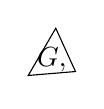
\begin{tikzpicture}[baseline=-.5ex]\node at (0,0) {$G$,};\draw (-.3,-.2)--(.3,-.15)--(.05,.4)--cycle;\end{tikzpicture}}
$X$ and $Y$ are algebraic schemes over $k$. If the action $\sigma$ is
\figure{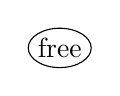
\begin{tikzpicture}[baseline=-.5ex]\node at (0,0) {free};\draw (0,0) ellipse (.4 and .25);\end{tikzpicture}},
and $(Y,\phi)$ is a geometric quotient of $X$ by $G$, then $X$ is a principal fibre bundle over $Y$ with group $G$.${}^*$

\margin{\figure{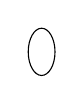
\begin{tikzpicture}\draw (0,0) ellipse (.17 and .3);\end{tikzpicture}}\unsure{Dangerous} \unsure{example}?}
\margin{\figure{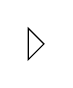
\begin{tikzpicture}\draw (0,0)--(.2,.2)--(0,.4)--cycle;\end{tikzpicture}}$G$ \uline{smooth}$/k$!}

\uline{Proof}: First of all, we may assume that $k$ is algebraically closed: for by such a base extension, i) $\sigma$ remains free, ii) $(Y,\phi)$ remains a geometric quotient (Remark $\unsure{\gamma|7}$, \S2), iii) the property of being a principal fibre bundle descends (SGA 8, 5.4). Secondly, we may replace $Y$ by one of its local rings $\operatorname{Spec}(\underline{o}_{y,Y})$, for some closed point $y\in Y$: for all conditions of Definition 0.10 are expressible locally. And thirdly, we may replace $\operatorname{Spec}(\underline{o}_{y,Y})$ by $\operatorname{Spec}(\hat{\underline{o}}_{y,Y})$ (its completion). For this is also a faithfully flat quasi-compact base extension and, as before, i) $\sigma$ remains free, ii) $(Y,\phi)$ remains a geometric quotient, and iii) the property of being a principal fibre bundle descends.

Therefore we have $Y=\operatorname{Spec}(A)$, where $A$ is a complete local ring with algebraically closed residue field. Let $y$ be the closed point of $Y$, and let $x$ be a closed, hence $k$-rational point of $X$ over $y$. Let $I_x\subset\underline{o}_{x,X}$ be
\figure{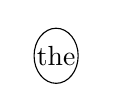
\begin{tikzpicture}[baseline=-.5ex]\node at (0,0) {the};\draw (0,0) ellipse (.28 and .35);\end{tikzpicture}}
ideal defining
\figure{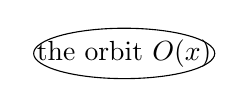
\begin{tikzpicture}[baseline=-.5ex]\node at (0,0) {the orbit $O(x)$};\draw (0,0) ellipse (1.15 and .32);\end{tikzpicture}}
of $x$. Since $\sigma$ is free, the morphism $\psi_x$ defines an isomorphism:
\[
\underline{o}_{x,X}/I_x\xrightarrow{\sim}\underline{o}_{e,G}.
\]
\margin{ambiguous}

\noindent\rule{2cm}{.4pt}

${}^*$It seems very likely that this result holds even if we do not assume \uline{a priori} that $Y$ is an algebraic scheme; and that it then follows \uline{a posteriori} that $Y$ is an algebraic scheme.

\margin{56}

\scanpage{58}

Considérons le composé
\[
\Delta^*j:\quad\underline{\operatorname{NS}}_{A/S}\deleted{(A)}\longrightarrow\unsure{P|\operatorname{Pic}}_{A/S}
\]
on sait que son composé avec $\unsure{P|\operatorname{Pic}}_{A/S}\xrightarrow{h}\underline{\operatorname{NS}}_{A/S}$ est $2\operatorname{id}_{\underline{\operatorname{NS}}_{A/S}}$. Donc \uline{le double de l'extension canonique de $\underline{\operatorname{NS}}_{A/S}$ par $P_{A/S}$ splitte canoniquement.}

\figure{\begin{tikzpicture}\draw (0,0) .. controls (2,0) and (2,.2) .. (2,.7) .. controls (2,1) and (2.4,1) .. (3,1) -- (9,1.1);\end{tikzpicture}}

Considérons d'autre part la restriction de $j'(h\Delta^*)\deleted{\unsure{j}}$ à $\underline{\operatorname{Tors}\,\mathrm{birig}\,\mathrm{sym}}(A,A;C)$.
Je dis que c'est la multiplication par $2$, i.e.
\[
h\Delta^*
\]

\margin{57}

\scanpage{59}
\mspage{-0.26 bis-}

Putting these two results together, it follows that if $G$ is reductive and the stabilizers are \uline{finite}, $\phi$ being affine is, in essence, a weak topological restriction, i.e. it is equivalent to the properness of $\sigma$. But if the stabilizers are positive dimensional, $\phi$ being affine is a much stronger restriction. At least in characteristic 0, it implies that these stabilizers are themselves reductive groups (cf. Iwahori [\quad]).

The final ``preliminary'' result is aimed at further motivating the concept of a geometric quotient by showing that, for a free action, it implies all that one might hope for.

\uline{Definition 0.10}: Let $(Y,\phi)$ be a geometric quotient of $X$ by $G$ (over $S$). Assume that $G$ is flat and of finite type over $S$. Then $X$ is a \uline{principal fibre bundle} over $Y$, with group $G$, if

\qquad i) $\phi$ is a flat morphism of finite type,

\qquad ii) $\unsure{\bar\psi|\bar\Psi}$ is an isomorphism of $G\mathbin{\underset{S}{\times}}X$ and $X\mathbin{\underset{Y}{\times}}X$.

\margin{58}

\scanpage{60}

``Th. des cycles invariants'':

Cas du $H^1$

\margin{59}

\scanpage{61}

Le résultat qui suit, qui résoud le``problème du cycle invariant'' dans le cas du $H^1$, est essentiellement une reformulation d'un résultat de M.RAYNAUD [\quad]:
\margin{$\times$}

\uline{Théorème} / Soient $S$ un trait strictement local, $f:X\unsure{\longrightarrow|\mathbin{-}}S$ un schéma \deleted{propre}\inserted{projectif} sur $S$, régulier, tel que l'on ait $\underline{O}_S\xrightarrow{\sim}f_*(\underline{O}_X)$, (ce qui implique que $X$ est plat sur $S$, et que $X_0$ est un diviseur sur $X$), \deleted{\unsure{soient $(D_i)_{i\in J}$ les}}\inserted{$(D_i)_{i\in J}$ la famille des} composantes irréductibles réduites de $X_0$, considérées comme diviseurs sur $X$, et posons \unsure{$\times$}
\[
(1)\qquad X_0=\sum_{i\in J}d_iD_i,\qquad\text{où }d_i\geq1,
\]
\[
(2)\qquad d=\operatorname{pgcd}(d_i)_{i\in J}.
\]
Soient
\[
(3)\qquad\Delta\simeq\underline{Z}^{J}
\]
la catégorie des diviseurs $D$ sur $X$ tels que $\operatorname{supp}D\subset X_0$, \deleted{et}
\[
(4)\qquad\deleted{\unsure{Ixx\underline Z}}\ \Gamma\simeq/\underline Z\cdot X_0\hookrightarrow\operatorname{Pic}(X)
\]
le \deleted{\unsure{cat}} sous-groupe de $\operatorname{Pic}(X)$ image de $\Delta$ par l'homomorphisme $D\mapsto\operatorname{cl}(\underline{O}_X(D))$ de $\Delta$ dans $\operatorname{Pic}(X)$, et considérons l'homomorphisme \deleted{composé}
\[
(5)\qquad w:\Gamma\longrightarrow\operatorname{NS}(X_0)\overset{\mathrm{dfn}}{=}\operatorname{Im}(\operatorname{Pic}(X_0)\longrightarrow\underline{\operatorname{NS}}_{X_0/k}(k)),
\]
composé des homomorphismes évidents
\diagram{\begin{tikzcd}
\Gamma\arrow[r,hook,"i"]&\operatorname{Pic}(X)\arrow[r]&\operatorname{Pic}(X_0)\arrow[r]&\operatorname{NS}(X_0).
\end{tikzcd}}
Soit enfin $d^t$ le pgcd des degrés des 0-cycles sur $X_\eta$. Avec ces notations, on a ce qui suit:

a) L'entier $d^t$ est aussi égal au pgcd des $\mu_i d_i$, où pour tout $i\in J$, $\mu_i$ désigne la multiplicité radicielle de $D_i$ sur $k$ (EGA IV 4.\quad); en particulier \deleted{$d$ divise $d^t$, donc est égal à 1 si $d^t$ l'est}\deleted{, \unsure{la réciproque étant vraie si $k$ est parfait}}\deleted{\inserted{et lui est égal si $k$ est parfait.}}\inserted{on a $d^t=p^h d$, où $p^h=\operatorname{pgcd}(\mu_i)$,}
\margin{\unsure{donc} $h=0$ i.e. $d=d^t$ si $k$ est parfait}
\margin{$\times$}

b) L'homomorphisme $w$ est un homomorphisme de $\underline Z$-modules \uline{de type fini dont le noyau est contenu dans le sous-groupe de torsion de $\Gamma$}. Ce dernier est isomorphe canoniquement à $\underline Z/d\underline Z$, avec comme générateur l'image dans $\Gamma$ du cycle $(1/d)X_0=\sum_{i\in J}(d_i/d)D_i$. Donc $\operatorname{Ker}w$ est cyclique

\margin{\figure{\begin{tikzpicture}\draw (0,8)--(0,0)--(.4,0);\draw[->](-.4,-.5)--(.4,0);\draw (0,-1)--(0,-2.3);\draw (-.7,8.3)--(-.4,8.9);\end{tikzpicture}}}
\margin{60}

\scanpage{62}

d'ordre \inserted{$d'$} divisant $d$, et a fortiori $d^t$.

c) \deleted{Pour tout} Soit $n$ un entier, et supposons que $n$ est premier à $p$, \uline{ou} que \inserted{$\unsure{d_t|d^t}$ est premier à $p$, ou que} $k$ est parfait(donc algébriquement clos).On a alors une suite exacte canonique, fonctorielle en $X$:
\diagram{\begin{tikzcd}[column sep=small]
(6)\quad 0\arrow[r]&{}_n\Gamma\arrow[r]\arrow[d,equal]&H^1(X,\mu_n)\arrow[r,"u_n"]&H^1(X_{\bar\eta},\mu_n)^I\arrow[r]&\operatorname{Ker}\deleted{{}_{\unsure{n}}}w_n\arrow[r]&0,\\
&\inserted{\underline Z/(n,d)\underline Z}&&&&
\end{tikzcd}}
où
\[
w_n:\Gamma_n\longrightarrow\operatorname{NS}(X_0)_n
\]
est l'homomorphisme déduit de (5) par tensorisation par $\underline Z/n\underline Z$, \deleted{Pour $n$ variable \unsure{multiplier}} et où $u_n$ est l'homomorphisme canonique (\qquad). Pour $n$ variable multiplicativement, les suites exactes (6) forment un système projectif de suites exactes, pour les morphismes de transition évidents.

\margin{$\times\quad\times\quad\times$}

d) Soit $\ell$ un nombre premier, \deleted{et supposons $\ell\neq p$ ou $k$ parfait.}\deleted{\inserted{ou $d_t$ premier à $p$ ou}} Alors on \deleted{trouve}\inserted{a} une suite exacte canonique, \inserted{fonctorielle en $X$} \deleted{(obtenue, si $\ell$ satisfait \inserted{aux conditions de c)}, par passage à la limite projective sur les puissances de $\ell$ dans les suites exactes (6)):}\deleted{on trouve une suite exacte}
\diagram{\begin{tikzcd}[column sep=small]
(7)\quad0\arrow[r,dash]&H^1(X,\underline Z_\ell(1))\arrow[r,"u(\ell)"]&H^1(X_{\bar\eta},\underline Z_\ell(1))^I\arrow[r]&R\otimes\underline Z_\ell\arrow[r]&0,
\end{tikzcd}}
où $R=\operatorname{Ker}w\simeq\underline Z/d'\underline Z$, donc
\[
(8)\qquad R\otimes\underline Z_\ell\simeq
\begin{cases}
0\text{ si }\ell\nmid d',\quad\inserted{\text{a fortiori si }\ell\nmid d^t,}\\
\underline Z/\ell\underline Z\text{ si }\ell\mid d'.
\end{cases}
\]
\margin{\figure{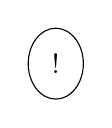
\begin{tikzpicture}\node at (0,0) {!};\draw (0,0) ellipse (.35 and .45);\end{tikzpicture}}}
\figure{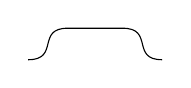
\begin{tikzpicture}\draw (0,0)..controls (.4,0) and (.1,.4)..(.5,.4)--(1.2,.4)..controls (1.6,.4) and (1.3,0)..(1.7,0);\end{tikzpicture}}

On obtient en particulier\unsure{*}, grâce à d): \deleted{du moins si $\ell\neq p$:}

\uline{Corollaire} \inserted{9}. \deleted{L'homomorphisme} Soit $\ell$ un nombre premier, \deleted{\unsure{tel que l'on ait $\ell\neq p$ si $k$ n'est pas parfait ou $d_t$}} Alors l'homomorphisme
\[
\inserted{(10)}\qquad u(\ell):H^1(X,\underline Z_\ell(1))\longrightarrow H^1(X_{\bar\eta},\underline Z_\ell(1))^I
\]
est injectif, son conoyau est un groupe fini, nul pour presque tout $\ell$.
La même conclusion est vraie en remplaçant $\underline Z_\ell(1)$ par $\underline Z_\ell$, à condition de supposer $\ell\neq p$.

\margin{$\times$}
\margin{\figure{\begin{tikzpicture}\draw (0,8)--(0,0);\draw (.2,-1)--(.2,-3);\end{tikzpicture}}}
\margin{61}

\scanpage{63}

Notons d'ailleurs, pour le cas d'un entier $n$ ne satisfaisant pas \inserted{nécessairement} les conditions envisagées dans c):

\uline{Corollaire} \inserted{10}. Soit $n$ un entier. On a alors une suite exacte canonique
\diagram{\begin{tikzcd}[column sep=small]
(\unsure{11|10})\quad0\arrow[r]&{}_n\Gamma\arrow[r]&H^1(X,\mu_n)\arrow[r,"u_n"]&H^1(X_{\bar\eta},\mu_n)^I\arrow[r]&Q\deleted{{}_n}(n)\arrow[r]&0,
\end{tikzcd}}
où $Q_n=\operatorname{Coker}u_n$ s'insère dans une suite exacte canonique
\diagram{\begin{tikzcd}[column sep=small]
(12)\quad0\arrow[r]&\operatorname{Ker}w_n\arrow[r]&Q\deleted{{}_n}(n)\arrow[r]&\theta(n)\arrow[r]&0,
\end{tikzcd}}
avec
\[
(13)\qquad\theta(n)\unsure{\hookrightarrow|\subset}{}_n\operatorname{Ker}(\operatorname{Br}(K)\longrightarrow\operatorname{Br}(X_\eta))\hookrightarrow{}_{(n,d^t)}\operatorname{Br}(K),
\]
\margin{\figure{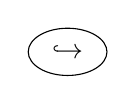
\begin{tikzpicture}\node at (0,0) {$\hookrightarrow$};\draw (0,0) ellipse (.5 and .3);\end{tikzpicture}}}
de sorte que l'on a $\theta(n)=0$ lorsque $n$ ou $d^t$ sont premiers à $p$ ou\deleted{\unsure{x}} que $k$ est parfait (donc $\operatorname{Br}(K)=0$). En tous cas, si $p^m$ est la plus grande puissance de $p$ divisant $d^t$ (qui est donc indépendant du choix de $n$), on a
\[
(14)\qquad p^m\theta(n)=0\qquad\text{pour tout }n.
\]
Pour $n$ variable multiplicativement, les \deleted{suites} diagrammes (\unsure{11|10}), (12) et (13) forment des systèmes projectifs, pour des morphismes de transition évidents, \deleted{et on a, \unsure{grâce grâce}}

Si donc $n$ parcourt lespuissances d'un nombre premier fixé $\ell$, alors il résulte de (14) que $\varprojlim_\nu\theta(\ell^\nu)=0$, \deleted{de sorte que par passage à la limite à partir des} donc $\varprojlim_\nu\operatorname{Ker}w_{\ell^\nu}\xrightarrow{\sim}\varprojlim Q(\ell^\nu)$ \deleted{et} par (12), d'où la suite exacte (7) par passage à la limite à partir de (\unsure{11|10}).

Nous prouverons également le

\uline{Corollaire} 15. Posons
\[
(16)\qquad d^{\unsure{t}}=p^r a,\qquad\text{avec }(a,p)=1.
\]
Alors il existe un \deleted{revêtement} diagramme
\diagram{\begin{tikzcd}
(17)\quad\unsure{X|M}\arrow[d,"f"']&X'\arrow[l,"h"']\arrow[d,"f'"]\\
S&S'\arrow[l,"g"]
\end{tikzcd}}
avec $h$ un revêtement étale \deleted{principal de groupe \unsure{G}}, $S'\longrightarrow S$ un revêtement

\margin{\figure{\begin{tikzpicture}\draw (0,0)--(0,6);\end{tikzpicture}}}
\margin{62}

\scanpage{64}

\unsure{kummérien|kumérien} \inserted{connexe} (ramifié) de \inserted{$S$, de} groupe de Galois $\mu_a$, le diagramme \deleted{étant} induit par le changement de base $\eta\longrightarrow S$ étant cartésien. Un tel diagramme est unique à isomorphisme près, \deleted{$X'$ est connexe,} et $f':X'\longrightarrow S'$ satisfait aux mêmes hypothèses \deleted{ici} que $f$ dans \qquad, mais l'entier $d(X'/S')$ (défini comme $d=d(X/S)$ dans (2)) est maintenant \deleted{une puissance} égal\deleted{\unsure{x}} à $p^r$.
Si $I'\subset I$ est le groupe d'inertie \deleted{\unsure{de}} relatif à $S'$, alors pour tout entier $n$ premier à $p$, \unsure{à}l'homomorphisme
\[
u'_n:H^1(X',\mu_n)\longrightarrow H^1(X_{\bar\eta},\mu_n)^{I'}
\]
est injectif, et son conoyau est isomorphe à $\deleted{\unsure{\Gamma}}{}_n\delta/{}_n\delta'$, où $\delta$ est le sous-groupe de torsion de $\operatorname{Coker}w$ ($w$ défini dans (5)) et $\delta'$ le sous-groupe de torsion de $\operatorname{NS}(X_0)$. On en conclut, pour tout nombre premier $\ell\neq p$, \deleted{une} que l'homomorphisme
\[
u'(\ell):H^1(X',\underline Z_\ell\deleted{(1)})\longrightarrow H^1(X'_{\bar\eta},\underline Z_\ell\deleted{(1)})^{I'}
\]
est un \uline{isomorphisme}.\deleted{\unsure{et la même conclusion}}

\margin{$\times\quad\times\quad\times$}
\margin{63}

\scanpage{65}

\margin{\fbox{$\unsure{N|\delta}\overset{\mathrm{dfn}}{=}\operatorname{Im}(\operatorname{Pic}(X_0)\longrightarrow\underline{\operatorname{NS}}_{X_0/k}(k))$}}
\uline{Théorème}\quad $S$ trait str. local

$X$ schéma propre sur $S$, régulier, tel que $\underline O_S\xrightarrow{\sim}f_*(\underline O_X)$, et que $X_\eta$ admette \inserted{un 0-cycle de degré 1}

$\Delta$ le groupe des diviseurs sur $X$ tels que $\operatorname{supp}\unsure{\Delta|D}\subset X_0$
\[
c:\Delta\mathbin{-}\deleted{\unsure{\operatorname{NS}(X_0)}}\ \underline{\operatorname{NS}}\deleted{\unsure{{}_{X_0/k}(k)}}(X_0)
\]
défini comme composé
\diagram{\begin{tikzcd}[column sep=small]
\Delta\arrow[r]&\operatorname{Pic}(X)\arrow[r,dash]&\operatorname{Pic}(X_0)\arrow[r,dash]&\underline{\operatorname{Pic}}_{X_0/k}(k)\arrow[r,dash]&\underline{\operatorname{NS}}_{X_0/k}(k)\arrow[r]&N
\end{tikzcd}}
\[
\left\{\begin{gathered}
\delta=\deleted{\unsure{\operatorname{Coker}c\text{ qui}}}\ \text{sous-groupe de torsion de }\operatorname{Coker}c,\\
\deleted{\unsure{\operatorname{NS}\text{ et }Z}\ \text{qui est le}\ \illegible{2}\ \operatorname{NS}(X_0),\ \text{de sorte que }\Delta\longrightarrow N\xrightarrow{\lambda}\delta\longrightarrow0}
\end{gathered}\right.
\]
\deleted{\unsure{Supposons}} Alors $\delta$ est un groupe \uline{fini}; \inserted{\unsure{torsion de} $\operatorname{NS}(X_0)=\delta'$, soit $\delta''=\delta/\delta'$} et pour tout entier $n$ premier à $p$, on a une suite exacte canonique
\diagram{\begin{tikzcd}[column sep=tiny,row sep=small]
(*)\quad\unsure{0}\arrow[r,dash]&H^1(X,\mu_n)\arrow[r,"u_n"]\arrow[d,equal]&H^1(X_{\bar\eta},\mu_n)^I\arrow[r]&\deleted{\unsure{{}_n\delta''}}\inserted{{}_n\delta/{}_n\delta'}\arrow[r]&\deleted{\unsure{\delta'}}\delta'_n\arrow[r]&\delta_n\arrow[r]&\delta''_n\arrow[r]&0\\
&\inserted{H^1(X_0,\mu_n)}&&\deleted{\unsure{\delta'}}&&&&
\end{tikzcd}}
compatible avec les morphismes de transition évidents en $n$, d'où par passage à la limite, pour tout $\ell$ nbr pr. $\neq p$
\[
H^1(X,\mathbb Z_\ell)\xrightarrow{\sim}H^1(X_{\bar\eta},\mathbb Z_\ell)^I
\]
(\uline{Théorème des cycles invariants}).
\margin{(\unsure{cas $X_i$})}

\uline{Dém} $X$ est plat sur $S$, donc $X_\eta$ dense ds $X$, et $H^1(X,\mu_n)\hookrightarrow H^1(X_\eta,\mu_n)$. On trouve le diagramme
\diagram{\begin{tikzcd}[column sep=small,row sep=large]
H^1(X,\mu_n)\arrow[r,"\alpha","\sim"']\arrow[d]&{}_n\operatorname{Pic}(X)\arrow[d]&&\\
H^1(X_\eta,\mu_n)/(\mathbb Z/n\mathbb Z)\arrow[r,"\alpha_\eta","\sim"']\arrow[d]&{}_n\operatorname{Pic}(X_\eta)\arrow[r,"\beta_\eta","\sim"']\arrow[d]&{}_nP(K)\arrow[r,equal]\arrow[d]&{}_nP(\bar K)^I\arrow[dl,bend left=20]\\
H^1(X_{\bar\eta},\mu_n)\arrow[r,"\alpha_{\bar\eta}","\sim"']&{}_n\operatorname{Pic}(X_{\bar\eta})\arrow[r,"\beta_{\bar\eta}","\sim"']&{}_nP(\bar K)&
\end{tikzcd}}
où $\alpha,\alpha_\eta,\alpha_{\bar\eta}$ sont des isom par \deleted{\unsure{suite exacte}} de Kummer et $f_*(\underline O_X)\simeq\underline O_S$ (\uline{NB} $V^*/V^{*n}=0$, $K^*/K^{*n}\simeq\mathbb Z/n\mathbb Z$, car $V$ \uline{str.} local) $\beta_\eta$ (et $\beta_{\bar\eta}$) \unsure{sont} isom à cause de l'existence d'un 0-cycle de degré 1 sur $X_\eta$, donc on voit que $u_n$ dans (*) s'identifie:
\[
(**)\qquad{}_nv:\quad{}_n\operatorname{Pic}(X)\mathbin{-}{}_n\operatorname{Pic}(X_\eta)
\]
Comme $X$ est régulier (il suffirait: anneaux locaux factoriels) on a
\diagram{\begin{tikzcd}
0\arrow[r]&\Gamma\arrow[r,"i"]&\operatorname{Pic}(X)\arrow[r,dash,"v"]&\operatorname{Pic}(X_\eta)\arrow[r]&0
\end{tikzcd}}
où $\Gamma=\Delta/\mathbb Z\cdot X_0$, d'où
\[
\operatorname{Coker}u_n\simeq\operatorname{Coker}{}_nv\simeq\operatorname{Ker}i_n,\quad\text{où }i_n:\Gamma_n\longrightarrow\operatorname{Pic}(X)_n
\]

\margin{64}

\scanpage{66}
\mspage{- 10 -}
\margin{n° 384}
$\unsure{\mathcal M|\mathfrak M}_+(G)$ (ch. IV, § 1, n° 1, prop. 4) et l'ensemble des $\alpha\in T$ telles que $\alpha(U)\leq 1$ est donc fermé. Il en résulte que l'ensemble $\Delta_U$ des $\alpha\in T$ satisfaisant à $\alpha(\{e\})\geq 1$ et à $\alpha(U)\leq 1$ est \uline{fermé} : remarquons que ces conditions sont équivalentes à $\alpha(\{e\})=\alpha(U)=1$ et par suite, $\Delta_U$ se compose exactement de l'\uline{ensemble des mesures de Haar normalisées des sous-groupes discrets} $H$ \uline{tels que} $H\cap U=\{e\}$ ; nous noterons $D_U$ l'ensemble de ces sous-groupes discrets.

Soit maintenant $\varphi$ une fonction de $\mathcal K_+(G)$, de support contenu dans $U$ et telle que $\varphi(e)=1$ : on a alors $\alpha(\varphi)=1$ pour toute $\alpha\in\Delta_U$, ce qui montre que $\Delta_U$ est contenu dans le \uline{compact} $T\cap L_\varphi$ (prop. 2) et est donc lui-même \uline{compact}. L'application canonique de $\Delta_U$ sur $D_U$ est donc un homéomorphisme et on a :

PROPOSITION 7.- \uline{Pour tout voisinage ouvert} $U$ \uline{de} $e$, \uline{l'ensemble} $D_U$ \uline{des sous-groupes discrets} $H$ \uline{de} $G$ \uline{tels que} $H\cap U=\{e\}$ \uline{est compact}.

Soit maintenant $V$ un autre voisinage ouvert de $e$, relativement compact et tel que $\overline V\subset U$ et soit $\varphi\in\mathcal K_+(G)$, de support contenu dans $U$ et avec $\varphi(x)=1$ pour $x\in V$. On a $\alpha(\varphi)=1$ pour $\alpha\in\Delta_U$ et il existe donc un voisinage $W$ de $\alpha$ dans $\Delta$ tel que $\beta(\varphi)<2$ pour $\beta\in W$ : on a alors $W\subset\Delta_V$, ce qui montre que $\Delta_V$ est un voisinage de $\Delta_U$. Par suite, les \uline{intérieurs} des sous-espaces $\Delta_U$ de $\Delta$ forment un recouvrement ouvert de $\Delta$ par des ensembles relativement compacts. On en déduit (compte tenu de ce que $\Delta_{U_1}\cap\cdots\cap\Delta_{U_n}=\Delta_{U_1\cap\cdots\cap U_n}$) :

PROPOSITION 8.- \uline{Le sous-espace} $\Delta$ \uline{de} $T$ \uline{est localement compact ; pour qu'une partie} $A$ \uline{de} $\Delta$ \uline{soit relativement compacte, il faut et il suffit qu'il existe un voisinage ouvert} $U$ \uline{de} $e$ \uline{tel que} $A\subset\Delta_U$.

Supposons maintenant que $G$ satisfasse à la condition suivante :

(L)\qquad il existe un voisinage $Q$ de $e$ tel que le seul sous-groupe \uline{discret} de $G$ contenu dans $Q$ soit le sous-groupe réduit à $\{e\}$.

En termes imagés, la condition (L) signifie que $G$ n'a pas de sous-groupes discrets arbitrairement petits. * On peut montrer que tout groupe de Lie satis-
\margin{65}

\scanpage{67}
\deleted{\unsure{Ainsi}}
\deleted{On sait que}
\deleted{On sait que}

On a d'autre part, si
\[
\deleted{0\longrightarrow\Gamma\longrightarrow}\qquad \unsure{j|j_0}:\Gamma\longrightarrow\operatorname{Pic}(X_0)\qquad\deleted{\unsure{\longrightarrow}}
\]
est le composé, d'où des $j_n:\Gamma_n\mathbin{-}\operatorname{Pic}(X_0)_n$, \deleted{\unsure{on a}} l'inclusion évidente :
\[
\operatorname{Ker}i_n\subset\operatorname{Ker}j_n.
\]
\margin{\uline{Lemme}. $\operatorname{Pic}(X)_n\longrightarrow\operatorname{Pic}(X_0)_n$ (du moins si $S$ complet, ce qui suffit pour le th.) \unsure{faisable par les th. clés}.}
Cette inclusion est \inserted{en fait} une \uline{identité}. Pour le voir, on note que si $L$ est un faisceau inv. sur $X$, et si $L_0=L|X_0$ est écrit comme puissance $n$ième, alors l'obstruction à écrire $L$ lui-même puissance $n$ième est nulle (cf \unsure{FGA|SGA}, exposé sur Picard). On a d'autre part
\[
\operatorname{Pic}(X_0)=\underline{\operatorname{Pic}}_{X_0/k}(k)
\]
\unsure{grâce} au fait que $X_0$ a un cycle de degré 1, d'où
\diagram{\begin{tikzcd}[column sep=large]
0\arrow[r,dash]&\operatorname{Pic}^{0}(X_0)\arrow[r,dash]\arrow[d,equal,"\mathrm{dfn}"']&\operatorname{Pic}(X_0)\arrow[r]&\operatorname{NS}(X_0)'\arrow[r]\arrow[d,equal,"\mathrm{dfn}"']&0\\
&\underline{\operatorname{Pic}}^{0}_{X_0/k}(k)&&\operatorname{Im}\bigl(\underline{\operatorname{Pic}}_{X_0/k}(k)\longrightarrow\underline{\operatorname{NS}}_{X_0/k}(k)\bigr)
\end{tikzcd}}
et $\operatorname{Pic}^{0}(X_0)$ est $n$-divisible, donc on a
\[
\operatorname{Pic}(X_0)_n\longrightarrow\operatorname{NS}(X_0)_n.
\]
\margin{\unsure{joindre au lemme précédent}}
donc si
\[
\unsure{k}:\Gamma\mathbin{-}\operatorname{NS}(X_0)
\]
est le composé $\Gamma\xrightarrow{j}\operatorname{Pic}(X_0)\longrightarrow\operatorname{NS}(X_0)$, on trouve
\[
\operatorname{Coker}u_n\simeq\operatorname{Ker}\unsure{k_n}.
\]
Je dis que \inserted{$\Gamma$ est sans torsion et que} $\unsure{k|\delta}$ est \uline{injectif}, i.e. qu'un faisceau inv. sur $X$ qui est trivial sur $X_\eta$, et qui sur $X_0$ est \deleted{\unsure{num.}} équiv. à zéro, est trivial.
\margin{cf plus bas une démonstration}
\inserted{$\unsure{L^l\simeq\mathcal O}\ \unsure{par l'imp.}$}
\deleted{\unsure{dans} $\operatorname{NS}(X_0)$ est nulle \unsure{implique par le critère (ou négativité) que} \unsure{pour ce est impossible le diviseur} \unsure{par} $\unsure{l\ne p}$, \unsure{et il peut faire le diviseur de} \unsure{fibre générique, en prenant dans} \unsure{Hensélisé un trait, on trouvera}}
\figure{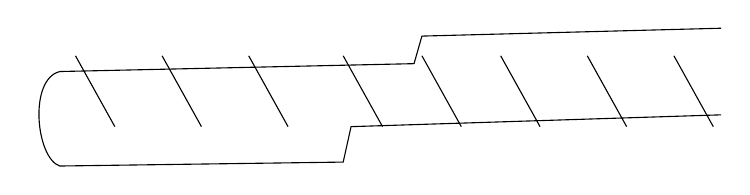
\begin{tikzpicture}[x=1cm,y=1cm]
\draw (0,1.4)--(4.5,1.5)--(4.6,1.85)--(8.4,1.95);\draw (0,1.4) .. controls (-.4,1.3) and (-.3,.3) .. (0,.2)--(3.6,.25)--(3.7,.7)--(8.4,.85);
\foreach \x in {.2,1.3,2.4,3.6,4.6,5.6,6.7,7.8}{\draw (\x,1.6)--(\x+.5,.7);}
\end{tikzpicture}}
une suite exacte
\deleted{\diagram{\begin{tikzcd}
0\arrow[r,dash]&\Gamma\arrow[r,"\unsure{k}",dash]&\operatorname{NS}(X_0)'\arrow[r,dash]&\unsure{\delta}\arrow[r]&0
\end{tikzcd}}}
\deleted{$\unsure{\operatorname{Coker}k=\operatorname{Coker}\Delta}$}
\deleted{$\unsure{\operatorname{Coker}\Delta}$}
\inserted{\diagram{\begin{tikzcd}[column sep=small]
0\arrow[r]&\Gamma\arrow[r,"k'"]&\operatorname{NS}(X_0)'\arrow[r,"\lambda"]\arrow[d,equal]&\delta\arrow[r]&0\\
&&\text{\unsure{sous-groupe de} }\operatorname{NS}(X_0)\text{ \unsure{dont un multiple donne dans} }\Gamma
\end{tikzcd}}}
d'où par le \unsure{sens} habituel
\[
\deleted{\unsure{donc}}\quad \operatorname{Ker}k_n=\operatorname{Ker}k'_n\simeq\operatorname{Coker}{}_n\lambda.
\]
Comme $\Gamma$ est sans torsion, \deleted{\unsure{on}} $\delta'\xrightarrow{\lambda}\delta$ est injectif, et on trouve que $\operatorname{Coker}{}_n\lambda={}_n\delta/{}_n\delta'$. On termine grâce à la suite
\margin{66}

\scanpage{68}
\mspage{- 9 -}
\margin{n° 384}
Puisque $Q_\alpha$ est compact, la constante 2 appartient à $\mathcal K_+(Q_\alpha)$ et il existe une fonction $g\in\mathcal K_+(G)$ avec $g*\alpha(x)=2$ pour tout $x\in G$. Soit $K$ le support de $g$ et posons $L=DK$. Il existe un voisinage $W$ de $\alpha$ dans $T^\circ$ tel que $g*\beta(x)\geq 1$ pour $x\in L$ et $\beta\in W$. Soit $\beta\in W$. Comme le support de $g*\beta$ est contenu dans $KH_\beta$, on a donc $DK\subset KH_\beta$. Supposons démontré que $D^{r-1}K\subset KH_\beta$ : on a alors :
\[
(14)\qquad D^rK=DD^{r-1}K\subset DKH_\beta\subset KH_\beta H_\beta=KH_\beta.
\]
Comme $G$ est la réunion des $D^r$, on en déduit que $G=KH_\beta$. De plus, on a $g*\beta\geq 1$ sur $K$ et $g*\beta$ est invariante à droite par $H_\beta$ : on a donc $g*\beta\geq 1$ partout et ceci montre que $W\subset T^\circ(g)$. Donc $T^\circ(g)$ est bien un voisinage de $\alpha$ et il est clair que $\beta\in T^\circ(g)$ entraîne $G=KH_\beta$ et par suite que $G/H_\beta$ est compact.

COROLLAIRE 1.- \uline{L'ensemble} $T^c$ \uline{des} $\alpha\in T^\circ$ \uline{telles que} $G/H_\alpha$ \uline{soit compact est un ouvert de} $T^\circ$ \uline{et la restriction de} $v$ \uline{à} $T^c$ \uline{est continue}.

COROLLAIRE 2.- \uline{L'ensemble} $S^c$ \uline{des sous-groupes fermés unimodulaires à quotient compact est un sous-ensemble ouvert de l'ensemble compact} $S^\circ$ \uline{des sous-groupes} \inserted{\uline{fermés unimodulaires}}.

La proposition 6 n'est pas exacte si on ne suppose pas que $G$ est engendré par un compact (exerc.\ ).

7. \uline{Sous-groupes discrets}.

Soit $D$ le sous-espace de $S$ formé des sous-groupes \uline{discrets} de $G$ et soit $\Delta$ le sous-espace de $T$ formé des mesures de Haar \uline{normalisées} des éléments de $D$ : pour qu'un élément $\alpha\in T$ appartienne à $\Delta$, il faut et il suffit que $\alpha(\{e\})=1$. On a évidemment $D\subset S^\circ$ et $\Delta\subset T^\circ$.

Pour tout compact $K$ de $G$, l'application $\alpha\longrightarrow\alpha(K)$ est semi-continue \uline{supérieurement} sur $\unsure{\mathcal M|\mathfrak M}_+(G)$ (ch. IV, § 4, n° 4, Remarque). Par suite l'ensemble des $\alpha\in T$ telles que $\alpha(\{e\})\geq 1$ est \uline{fermé} dans $T$. D'autre part, pour tout voisinage ouvert $U$ de $e$, l'application $\alpha\longrightarrow\alpha(U)$ est semi-continue inférieurement sur
\margin{67}

\scanpage{69}
exacte
\[
0\mathbin{-}\delta'\mathbin{-}\delta\mathbin{-}\delta''\mathbin{-}0
\]
et la suite exacte associée
\[
0\mathbin{-}{}_n\delta'\mathbin{-}{}_n\delta\mathbin{-}{}_n\delta''\mathbin{-}\delta'_n\mathbin{-}\delta_n\mathbin{-}\delta''_n.
\]
Reste à prouver : \textcircled{a}) le fait que $\Gamma$ est sans torsion. Mais $\unsure{\Gamma|\Gamma_{\mathrm{tors}}}=\mathbf Z/d\mathbf Z$, où $d$ est le pgcd des $d_i$, $X_0=\sum d_iD_i$, \& $X_{0\mathrm{red}}=\sum\unsure{D_i}$. \deleted{On voit que si $\exists$ sur $X$ un cycle \unsure{un cycle} de degré 1} si on a un pt fermé $x$ de $X_\eta$, son adhérence \inserted{\unsure{schématique dans} $X$} est un sous-schéma \inserted{fermé $Z$} \deleted{plat} de $X$, plat et fini sur $S$, \deleted{qui est} dont le degré sur $S$ est aussi égal à la multiplicité d'intersection \inserted{$Z.X_0$} sur $X$, qui est $\sum d_iZ.D_i$, donc multiple de $d$. Donc si $d'\deleted{\unsure{d}}$ est le pgcd des degrés des 0-cycles sur $X_\eta$, on a $d\mid d'$. Comme $d'=1$, on a $d=1$.
\margin{\uline{donner lemme} (ici \unsure{est} $X$ régulier, \unsure{substantiel})}

\textcircled{b}) $\Gamma\longrightarrow\operatorname{NS}(X_0)$ est \uline{injectif}.
\margin{\uline{donner \unsure{corollaire}} \uline{th.}}
[\unsure{Si est} $R$ son noyau, \inserted{qui est $\mathbf Z$ libre et t.t. \unsure{p. 0}}, \deleted{On} a la suite exacte
\[
0\mathbin{-}\mathrm H^1(X,\mu_n)\longrightarrow\mathrm H^1(X_{\bar\eta},\mu_n)^I\longrightarrow\unsure{{}_n\Gamma_n|\Gamma_n}\mathbin{-}\operatorname{NS}(X_0)_n
\]
d'où, par passage à la limite sur les puissances d'un $\ell$
\[
0\mathbin{-}\mathrm H^1(X,\mathbf Z_\ell(1))\mathbin{-}\mathrm H^1(X_{\bar\eta},\mathbf Z_\ell(1))^I\longrightarrow\unsure{\widehat{T}_\ell(\Gamma)\otimes\mathbf Z_\ell|\Gamma\otimes\mathbf Z_\ell}\mathbin{-}\unsure{\widehat{T}_\ell(\operatorname{NS}(X_0))\otimes\mathbf Z_\ell|\operatorname{NS}(X_0)\otimes\mathbf Z_\ell}
\]
i.e. on trouve, comme $\deleted{\unsure{T_\ell R\simeq}}R\otimes\mathbf Z_\ell\simeq\operatorname{Ker}(\Gamma\otimes\mathbf Z_\ell\mathbin{-}\operatorname{NS}(X_0)\otimes\mathbf Z_\ell)$
\deleted{$\unsure{T_\ell R}$}\quad\unsure{$\rho$}
\[
0\mathbin{-}\mathrm H^1(X,\mathbf Z_\ell(1))\mathbin{-}\mathrm H^1(X_{\bar\eta},\mathbf Z_\ell(1))^I\mathbin{-}R\otimes\mathbf Z_\ell\mathbin{-}0.
\]
Donc notre assertion équivaut à dire que l'on a la formule des cycles invariants ; \deleted{\unsure{comme}} il suffit de la prouver à torsion près.]
\margin{[\quad] en remarque après le cor.}

\deleted{L'idée est de se ramener au cas où $X$ est de dim relative un. Dans ce cas, on sait que $\unsure{\Gamma}$ est nul ($\unsure{D_i.D_j}$, c'est le fait que \unsure{son associé} matrice \inserted{d'intersection} est de rang $\unsure{r-1}$, où $r$ est le nb de composantes $D_i$).}
\figure{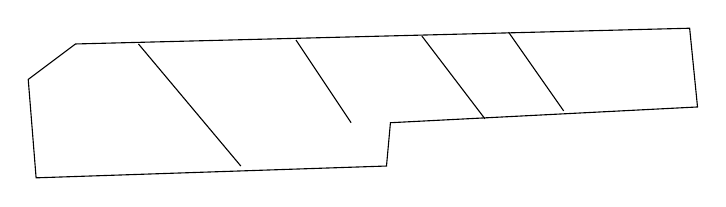
\begin{tikzpicture}[x=1cm,y=1cm]
\draw (0,1.4)--(.6,1.85)--(8.4,2.05)--(8.5,1.05)--(4.6,.85)--(4.55,.3)--(.1,.15)--(0,1.4);
\draw (1.4,1.85)--(2.7,.3);\draw (3.4,1.9)--(4.1,.85);\draw (5.0,1.95)--(5.8,.9);\draw (6.1,2)--(6.8,1);
\end{tikzpicture}}
Or c'est fait par Raynaud dans sa note : spécialisation des foncteurs de Picard, \uline{th. 3} --- dans version sans \deleted{\unsure{dans}} hyp. projective.
\margin{\unsure{donner dém. directe, en cas de dim. rel. 1}}
\deleted{[\unsure{Le fait le plus simple que} $\unsure{R^I}$ \unsure{est} \illegible{3} \unsure{se ramène} \illegible{5}]}
\figure{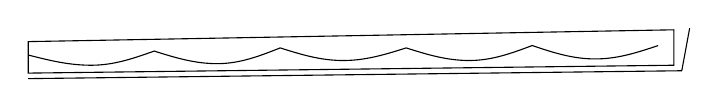
\begin{tikzpicture}[x=1cm,y=1cm]
\draw (0,0)--(8.2,.1)--(8.2,.55)--(0,.4)--cycle;
\draw (0,.23) sin (.8,.1) cos (1.6,.28) sin (2.4,.12) cos (3.2,.32) sin (4,.16) cos (4.8,.32) sin (5.6,.16) cos (6.4,.35) sin (7.2,.18) cos (8,.35);
\draw (0,-.07)--(8.3,.03);\draw (8.3,.03)--(8.4,.57);
\end{tikzpicture}}
\margin{68}

\scanpage{70}
\mspage{- 7 -}
\margin{n° 384}
sur $T^\circ$ et est strictement positive pour $f\ne 0$. Par suite, $v$ est enveloppe supérieure de fonctions continues et est donc semi-continue inférieurement.

Soit maintenant $g$ une fonction numérique positive, $\mu$-intégrable sur $G$. D'après la prop. 5 du ch. VII, § 2, la fonction $g^{b(\alpha)}$ sur $Q_\alpha$ définie par
\[
g^{b(\alpha)}\circ\varpi_\alpha(x)=\int^*g(xs)\,d\alpha(s)
\]
est finie presque partout (pour $\mu/\alpha$) et est $\mu/\alpha$-intégrable ; de plus, on a $\mu(g)=(\mu/\alpha)(g^{b(\alpha)})$.

PROPOSITION 5.- \uline{Soit} $g$ \uline{une fonction numérique positive} $\mu$-\uline{intégrable sur} $G$ \uline{et soit} $T^\circ(g)$ \uline{l'ensemble des} $\alpha\in T^\circ$ \uline{telles que} $\inf g^{b(\alpha)}\geq 1$. \uline{La restriction de} $v$ \uline{à} $T^\circ(g)$ \uline{est continue}.

D'après la prop. 4, il suffit de montrer que la restriction de $v$ à $T^\circ(g)$ est semi-continue supérieurement. Soit donc $\unsure{\Phi|\mathfrak F}$ un filtre sur $T^\circ(g)$, convergeant vers un point $\alpha\in T^\circ(g)$. Soit $\varepsilon$ un nombre réel $>0$ et soit $h\in\mathcal K_+(G)$ avec $\mu(|g-h|)<\varepsilon$. Soit $K$ le support de $h$ et soit $F$ une fonction de $\mathcal K(Q_\alpha)$, comprise entre 0 et 1, avec $F=1$ sur le compact $\varpi_\alpha(K)$. Il existe une fonction $f\in\mathcal K_+(G)$ avec $f^{b(\alpha)}=F$ (ch. VII, § 2, n° 1, prop. 2) : on a donc $f*\alpha\leq 1$ partout et $f*\alpha=1$ sur $K$. De plus, pour tout $\beta\in T^\circ$, on a :
\[
(10)\qquad v(\alpha)\geq\mu/\alpha(F)=\mu/\alpha(f^{b(\alpha)})=\mu(f)=(\mu/\beta)(f^{b(\beta)})
\]
et $f^{b(\beta)}\circ\varpi_\beta=f*\beta$. Les propriétés de continuité de l'application $\beta\longrightarrow f*\beta$ montrent qu'il existe un ensemble $A\in\unsure{\Phi|\mathfrak F}$ tel que $f*\beta(x)>1-\varepsilon$ pour tout $x\in K$ et $\beta\in A$. Si $\beta\in A$, on a donc $f^{b(\beta)}>1-\varepsilon$ sur $\varpi_\beta(K)$ et par suite :
\[
(11)\qquad (\mu/\beta)(f^{b(\beta)})>(1-\varepsilon)(\mu/\beta)(\varpi_\beta(K)).
\]
Posons $X_\beta=Q_\beta-\varpi_\beta(K)$ et $Y_\beta=\varpi^{-1}(X_\beta)$ : on a $K\subset G-Y_\beta$ et $h=0$ sur $Y_\beta$.
Soit $\varphi_\beta$ (resp. $\psi_\beta$) la fonction caractéristique de l'ouvert $X_\beta$ (resp. $Y_\beta$) ; on a :
\margin{69}

\scanpage{71}
\uline{Variante} laissons tomber l'hypothèse $d'\ (=\mathrm{pgcd}\text{ des deg. des 0-cycles sur }X_\eta)=1$.
On sait que $\operatorname{Br}(K)$ est un grpe de $p$-torsion, donc on a
\[
0\longrightarrow\operatorname{Pic}(X_\eta)\mathbin{-}P(K)\mathbin{-}\Theta\mathbin{-}0,
\]
où $\Theta\subset\operatorname{Br}(K)$ est un grpe de $p$-torsion, d'où résulte que ${}_n\operatorname{Pic}(X_\eta)\simeq{}_nP(K)$. Donc il reste vrai que $u_n$ est isom. à ${}_nv$. Mais $\Gamma$ peut avoir de la torsion. On trouve
\diagram{\begin{tikzcd}[column sep=small]
0\arrow[r]&{}_n\Gamma\arrow[r]\arrow[d,"\unsure{\simeq}"']&\mathrm H^1(X,\mu_n)\arrow[r,dash]&\mathrm H^1(X_{\bar\eta},\mu_n)^I\arrow[r]&\Gamma_n\arrow[r,dash]&\operatorname{NS}(X_0)_n\arrow[r]&{}\\
&\mathbf Z/(n,d)\mathbf Z
\end{tikzcd}}
\deleted{\unsure{Soit}} et par passage à la limite sur les puissances de $\ell$
\diagram{\begin{tikzcd}[column sep=small]
0\arrow[r,dash]&\mathrm H^1(X,\mathbf Z_\ell(1))\arrow[r]&\mathrm H^1(X_{\bar\eta},\mathbf Z_\ell(1))^I\arrow[r]\arrow[dr]&\Gamma\otimes\mathbf Z_\ell\arrow[r,dash]&\operatorname{NS}(X_0)\otimes\mathbf Z_\ell\\
&&&R\otimes\mathbf Z_\ell\arrow[r,dash]&0
\end{tikzcd}}
$R=\operatorname{Ker}(\Gamma\mathbin{-}\operatorname{NS}(X_0))$.
\margin{N.B. $R\otimes\mathbf Z_\ell\simeq\begin{cases}\mathbf Z/\ell\mathbf Z&\text{si }\ell\mid d\\0&\text{sinon}\end{cases}$}
On sait aussi (tout au moins modulo rés. des singularités, \unsure{qu'on pourrait faire cas. de ce bon}) que le noyau $R$ de $\Gamma\mathbin{-}\operatorname{NS}(X_0)$ est de \uline{torsion}. \deleted{(donc un grpe cyclique \unsure{d'ordre diviseur de} $d$, $\unsure{\mathbf Z/d'\mathbf Z}$)} C'est donc un sous-grpe de $\operatorname{tors}\Gamma\simeq\mathbf Z/d\mathbf Z$, [avec une nette tendance d'être égal à $\mathbf Z/d\mathbf Z$ tout entier ; \deleted{\unsure{et}} tout au moins le noyau contient-il la partie de $\operatorname{tors}\Gamma$ première à $p$, \unsure{pt} argument de Raynaud utilisant un rev. étale convenable de $S$ $\ldots$) On a donc, si
\margin{\unsure{même sans résolution} cf \unsure{in} Raynaud \unsure{note}, \unsure{prop. 7 (ii)}}
\margin{demander Raynaud si $\operatorname{Ker}$ est donc $\mathbf Z/d\mathbf Z$}
\[
\Gamma'=\Gamma/T\deleted{\unsure{orsion}},\quad\deleted{\unsure{\&}}\quad T:\operatorname{Torsion}\text{ de }\Gamma
\]
\[
0\mathbin{-}T_n\mathbin{-}\Gamma_n\mathbin{-}\Gamma'_n\longrightarrow0
\]
d'où, choisissant un splitting de $\Gamma\mathbin{-}\Gamma'\oplus T$, on trouve
\[
\operatorname{Ker}(\Gamma_n\mathbin{-}\operatorname{NS}(X_0)_n)\simeq T_n+\underbrace{\operatorname{Ker}(\Gamma'_n\mathbin{-}\operatorname{NS}(X_0)_n)}_{\operatorname{Ker}(\overline\Gamma_n\mathbin{-}\operatorname{NS}(X_0)_n)}
\]
où $\overline\Gamma\subset\operatorname{NS}(X_0)$
\[
\overline\Gamma=\operatorname{Im}\Gamma.
\]
On trouve donc, comme $\overline\Gamma$ n'a plus que de la $p$-torsion
\diagram{\begin{tikzcd}[column sep=large]
0\arrow[r,dash]&\delta'\arrow[r]\arrow[d,equal]&\delta\arrow[r,dash]&\delta''\arrow[r,dash]&0\\
&\text{tors de }\operatorname{NS}(X_0)\text{ première à }p
\end{tikzcd}}
\margin{70}

\scanpage{72}
\mspage{- 3 -}
\margin{n° 384}
du support de $\alpha$. Soit $V$ un voisinage de $x$ et soit $A$ un élément de $\unsure{\Phi|\mathfrak F}$. Soit $\varphi$ une fonction de $\mathcal K_+(G)$, de support contenu dans $V$ et telle que $\alpha(\varphi)\ne 0$. Puisque $\unsure{\Phi|\mathfrak F}$ converge vers $\alpha$, il existe un élément $B$ de $\unsure{\Phi|\mathfrak F}$ tel que $\beta(\varphi)\ne 0$ pour $\beta\in B$. Par suite l'ensemble des $\beta\in A$ tels que $V\cap H_\beta\ne\varnothing$ n'est pas vide. Choisissons un tel élément $\beta(V,A)$ et choisissons un point $x(V,A)\in V\cap H_{\beta(V,A)}$. L'application $(V,A)\longrightarrow\beta(V,A)$ (resp. $x(V,A)$) converge vers $\alpha$ (resp. $x$) suivant le filtre des sections du filtre produit du filtre des voisinages de $x$ et du filtre $\unsure{\Phi|\mathfrak F}$ (ouf ! Vive les directed sets !). D'autre part, on a :
\[
(4)\qquad\beta(V,A)=\beta(V,A)*\varepsilon_{x(V,A)}.
\]
Mais les mesures $\varepsilon_{x(V,A)}$ décrivent un ensemble équicontinu $\unsure{\mathcal C|\mathcal E}'(G)$ lorsque $V$ décrit l'ensemble des voisinages de $x$ contenus dans un même voisinage compact. Compte tenu de ce que la topologie vague coïncide sur $\unsure{\mathcal M|\mathfrak M}_+(G)$ (resp. sur un ensemble équicontinu de $\unsure{\mathcal C|\mathcal E}'(G)$) avec la topologie de la convergence uniforme sur les compacts de $\mathcal K(G)$ (resp. de $\unsure{\mathcal C|\mathcal E}(G)$) (Int., ch. III, 2ième édit., § 1, $\ldots$), on déduit alors de (4) et de l'hypocontinuité de la convolution (§ 3, cor. à la prop. 12) que :
\[
(5)\qquad\alpha=\alpha*\varepsilon_x.
\]
Par suite, tout point $y$ de support $H_\alpha$ de $\alpha$ appartient aussi au support de $\alpha*\varepsilon_x$, c'est-à-dire à $H_\alpha x$. Par suite, $yx^{-1}$ appartient à $H_\alpha$ et comme $H_\alpha$ n'est pas vide, c'est un \uline{sous-groupe} de $G$. Enfin, (5) entraîne que la mesure induite par $\alpha$ sur $H_\alpha$ est une mesure de Haar à droite sur $H_\alpha$. Par suite, on a bien $\alpha\in T$.

3. \uline{Bases de} $T$.

Soit $\varphi\in\mathcal K_+(G)$, avec $\varphi(e)>0$. Soit $L_\varphi$ l'hyperplan $\mu(\varphi)=1$ dans $\unsure{\mathcal M|\mathfrak M}(G)$. Pour tout $\alpha\in T$, la restriction de $\varphi$ au sous-groupe $H_\alpha$ est un élément non nul de $\mathcal K_+(H_\alpha)$ et on a $\alpha(\varphi)>0$. Par suite, l'hyperplan $L_\varphi$ rencontre chaque géné-
\margin{71}

\scanpage{73}
Th. d'orthogonalité \inserted{(\unsure{partiel!|partiel})} pour les modèles de Néron : démonstration arithmétique
\margin{72}

\scanpage{74}
\uline{Un théorème d'orthogonalité}

\deleted{$X$ schéma}
$A$ anneau noethérien $J$-adique (séparé et complet)
\[
X=\operatorname{Spec}A\qquad
Y=\operatorname{Spec}(A/J)=V(J)
\]
\deleted{$\unsure{G}$}
\[
U=X-Y
\]
Pour tout schéma fini étale $Z$ sur $Y$, $\widetilde Z$ est le schéma fini étale sur $X$ (unique à isom unique près) le prolongeant.
\margin{\unsure{Idem} pour faisceaux $\ell$-adiques \unsure{constants tordus}, $\ldots$}
$G,G'$ schémas \deleted{\unsure{lisses}} \inserted{en groupes comm. \deleted{\unsure{séparés}} de t.f. séparés} \inserted{plats} sur $X$ \deleted{séparés}
\[
\begin{array}{ll}
G_U=G|U&\text{est un schéma abélien }A\\
G'_U=G'|U&\text{\rule{5cm}{.3pt}}\quad A'
\end{array}
\]
\margin{$A$ et $A'$ \deleted{\unsure{duaux l'un de l'autre}} \inserted{accouplés}, i.e. on a un élém. de corr. alg. sur $A\times A'$.}
$\ell$ \deleted{\unsure{entier}} nb premier inv. sur $Y$, donc sur $X$.
\margin{\unsure{commencer par parler de} $\unsure{Z,Z'}$, \unsure{puis parler de} $\deleted{\unsure{G}}A,A'$}
$S\subset G_Y=G\times_XY$ est \inserted{plat sur $Y$ et} tel que ${}_{\ell^\nu}S$ \uline{fini} sur $Y$ pour tout $\nu>0$.
\deleted{$\unsure{S'\subset G'_Y=G'\times_XY}$ \unsure{avec} $\unsure{{}_{\ell^\nu}S'}$ \unsure{fini sur} $Y$}
\[
T'\subset G'_Y\qquad\text{un \uline{tore}}
\]
\deleted{\unsure{Alors}}
$\widetilde{T_\ell(S)}\deleted{\unsure{\subset}}$ est défini, et il est $\subset T_\ell(G)$
idem $\widetilde{T_\ell(T)}$ défini et $\subset T_\ell(G')$
\margin{\uline{NB} les ${}_{\ell^\nu}G$ sont étales de t.f. sép. sur $S$, et leur restriction à $Y$ contient les ${}_{\ell^\nu}S$, donc ${}_{\ell^\nu}G$ contient ${}_{\ell^\nu}\widetilde S$.}
\diagram{\begin{tikzcd}[row sep=small]
\widetilde{T_\ell(S)}|U\subset T_\ell(A)\\[-.4em]
\times\\[-.4em]
\widetilde{T_\ell(T)}|U\subset T_\ell(A')\arrow[d,"\varphi_\xi"']\\
T_\ell(\mathbf G_{mU})=\widetilde{T_\ell(\mathbf G_{mY})}|U
\end{tikzcd}}
\margin{$\xi$ induit $T_\ell(\xi)$}
\uline{Théorème}
\[
\varphi_\xi\bigl(\widetilde{T_\ell(S)}|U,\widetilde{T_\ell(T)}|U\bigr)=0
\]
\uline{Dém} Il suffit de le prouver en chaque pt $x\in U$.
Prenant un point \inserted{$y\in\overline{\{x\}}\cap Y$} \deleted{dans l'adhérence}, et dominant par un anneau de val. discret, on est ramené au cas où $X$ est un \uline{trait}, $Y$ son pt fermé, $U$ son pt gén. Il suffit d'ailleurs, dans cette réduction, de prendre pour $x$ un pt maximal de $U$. Supposons \deleted{que} d'abord qu'on
\margin{73}

\scanpage{75}
puisse, pour tt $x$, choisir $y\in\overline{\{x\}}\cap Y$ tel que $k(y)$ soit \uline{fini}. \inserted{(c'est le cas si $A/J$ de type fini sur $\mathbf Z$).} Alors par l'argument précédent, on est ramené au cas d'un \deleted{anneau de val. discrète} \inserted{localisé complété de} $X$ en $y$, \deleted{\unsure{donc }Y_0\unsure{\text{ en }y}}, donc $X$ local complet, de pt fermé $y$, de $k(y)$ fini. Alors $X-Y$ est de Jacobson, donc tte composante connexe de $X-Y$ a un pt $z$ tel que $\dim\overline{\{z\}}=1$, \uline{Soit} $Z=\overline{\{z\}}$ et $\unsure{\text{son}}$ l'adhérence dans $X$. Cela nous ramène, \deleted{\unsure{par un théorème}} quitte à remplacer $X$ par $Z$, au cas où $X$ local complet de dim 1, et en normalisant, au cas où $X$ est \inserted{le spectre d'} un anneau de valuation discrète $V$ à corps résiduel fini, $Y$ pt fermé. L'énoncé envisagé correspond alors à un homo de modules sur $\pi=\operatorname{Gal}(\overline K/K)$, ext. de $\pi_0\simeq\deleted{\unsure{\mathbf Z}}\operatorname{Gal}(\overline k/k)$ \inserted{$=\widehat{\mathbf Z}$} par le grpe d'inertie $I$.

\deleted{On peut supposer $T\simeq\mathbf G_{mk}^{r}$ (par extension résiduelle finie) et $T_\ell(\widetilde T)|U$ correspond à
\[
\deleted{T_\ell(\overline K^*)\simeq T_\ell(\overline k^*)}\quad (\widetilde{T_\ell(\mathbf G_{mk})}|U)^r\simeq T_\ell(\mathbf G_{m\overline K})^r\simeq T_\ell(\overline K^*)^r,
\]
comme module sur $\deleted{\mathbf Z_\ell}\pi_0$. D'autre part, pour $S$ on $T_\ell(S)$ \unsure{correspond}}
\figure{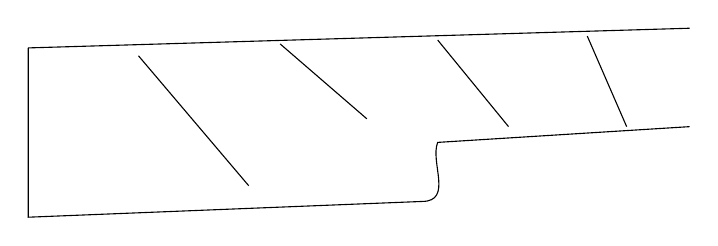
\begin{tikzpicture}[x=1cm,y=1cm]
\draw (0,2.3)--(8.4,2.55);\draw (0,2.3)--(0,.15)--(5,.35) .. controls (5.4,.35) and (5.1,.85) .. (5.2,1.1)--(8.4,1.3);
\draw (1.4,2.2)--(2.8,.55);\draw (3.2,2.35)--(4.3,1.4);\draw (5.2,2.4)--(6.1,1.3);\draw (7.1,2.45)--(7.6,1.3);
\end{tikzpicture}}
L'accouplement sur $U$, comme $X$ normal, provient d'un accouplement
\[
T_\ell(S)\times T_\ell(T)\mathbin{-}T_\ell(\mathbf G_{mk}).
\]
Donc dans ce cas on est ramené au

\uline{Lemme} Soit $k$ un corps fini, $S,\unsure{T'|T}$ deux grpes alg. commutatifs sur $k$, \deleted{dont le second est un tore} \inserted{où $T$ de t. mult.}. Alors tt. accouplement
\[
T_\ell(S)\times T_\ell(T)\mathbin{-}T_\ell(\mathbf G_m)
\]
est identiquement nul.
\margin{74}

\scanpage{76}
En effet, \deleted{\unsure{quitte}} on peut supposer \inserted{$S,T$ connexes réduits, donc $T$ un tore} \deleted{\unsure{déployés : par une extension} \inserted{finie} de $k$, \unsure{que} $T$ et le tore \unsure{maximal} $S_0$ de $S$}.
On peut supposer aussi $S$ extension d'une VA par un tore $S_0$. Quitte à faire une extension finie, on peut supposer
\[
S_0\simeq\mathbf G_m^r,\qquad T\simeq\mathbf G_m^s.
\]
Alors $T_\ell(S_0)\times T_\ell(T)\mathbin{-}T_\ell(\mathbf G_m)$ est un accouplement
\[
\mathbf Z_\ell^r\otimes\mathbf Z_\ell^s\mathbin{-}\mathbf Z_\ell^{\unsure{s|1}},
\]
où \deleted{$\unsure{\mathbf Z_\ell}$} l'élém. $f$ de Frob. opère sur \deleted{$\mathbf Z_\ell$} les trois facteurs par $q\,\mathrm{id},q\,\mathrm{id},q\,\mathrm{id}$, donc sur le premier \unsure{mb.} par $q^2\,\mathrm{id}$, sur le dernier par $q\,\mathrm{id}$. Donc l'accouplement induit est nul. Cela nous ramène au cas où $S$ est une V.A. Mais par Weil, les val. propres de $f$ opérant sur $\deleted{\unsure{\mathbf Z_\ell}}T_\ell(S)$ sont de val. absolue $q^{1/2}$, donc les val. propres sur $T_\ell(S)\otimes T_\ell(\mathbf G_m)$ sont de val. absolue $q^{3/2}$, et sur $T_\ell(\mathbf G_m)$ on a $q$, on a encore nullité.
\figure{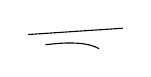
\begin{tikzpicture}\draw (0,0)--(1.2,.08);\draw (.22,-.13)..controls (.6,-.08) and (.8,-.12)..(.9,-.18);\end{tikzpicture}}

Nous traitons maintenant le cas général, \deleted{Pour cela}, \unsure{qui, nous le savons}, se ramène au cas $X$ un trait \inserted{$=\operatorname{Spec}V$, \unsure{de val. discr.}} $Y$ son pt fermé. On écrit
\[
V=\varinjlim A_i,\qquad A_i\subset V,\qquad A_i\deleted{\unsure{étant}}\text{ de t.f. sur }\mathbf Z.
\]
\deleted{\unsure{Pour ce faire}} Soit
\[
X_i=\operatorname{Spec}A_i,\quad Y_i=V(\unsure{\mathfrak p_i|p_i}),\quad U_i=X_i-Y_i;
\]
donc
\[
X=\varprojlim X_i,\quad Y=\varprojlim Y_i,\quad U=\varprojlim U_i.
\]
\margin{75}

\scanpage{77}
Pour $i$ grand $G,G'$ proviennent de $G_i,G'_i$ \inserted{sch. en grpes comm. de t.f. plats sur $X_i$}.
\deleted{et $\xi$ d'une corr.}
$G_i|U_i=A_i$ et $G'_i|U_i=A'_i$ des sch. abéliens, $\xi$ provient d'un élém de corr. div. $\xi_i$ sur $A_i\times A'_i$ ; $T$ provient d'un tore $T_i\subset G'_{iY_i}$, $S$ provient d'un sous-schéma plat $S_i\subset G_{iY_i}$.
De plus, \deleted{dans le cas} \deleted{\unsure{Encore}} on peut \deleted{\unsure{sans restriction}} supposer $S$ connexe \inserted{lisse} (sinon le remplacer par $S^0$) et \deleted{\unsure{de la partie unipotente} \unsure{Comme si} $\operatorname{car}k>0$ \unsure{comme le quotient par} $\unsure{p^nS}$} extension \deleted{d'une} successive d'une V.A., d'un tore \deleted{\unsure{pour }$S$\unsure{ propre et de un grpe}} grpe un. On peut donc supposer le même dévissage valable pour $S_i$.
\deleted{\unsure{Cela implique}}
On peut supposer enfin (remplaçant au besoin les $A_i$ par $A_i[1/\ell]$) que $\ell$ inv. sur les $X_i$, donc les $Y_i$. Mais les ${}_{\ell^\nu}S_i$ sont encore \unsure{finis|fini} sur $Y_i$. Bref, ttes les données proviennent de données analogues, avec un \deleted{$\unsure{X}$} $X_0$ \inserted{$=\operatorname{Spec}A_0$} \uline{de type fini} sur $\operatorname{Spec}\mathbf Z$.

De plus, si $\mathfrak p=\mathfrak m\cap A_0$, alors $A_0\mathbin{-}V$ induit $\widehat A_0\longrightarrow V$, \deleted{\unsure{comme}} Donc, on peut remplacer les mots ``$A_0$ de type fini sur $\operatorname{Spec}\mathbf Z$'' par ``$A_0$ $\mathfrak p$-adique séparé et complet, avec $A_0/\mathfrak p$ de t.f. sur $\operatorname{Spec}\mathbf Z$, et $A_0\mathbin{-}V$ continu pour les topologies adiques''. On est ramené alors au th. pour cet $X_0,Y_0,G_0,G'_0,\xi_0,S_0,T_0$, et il relève du cas 1.
\hfill CQFD.
\margin{76}

\scanpage{78}
INSTITUT

DES HAUTES ETUDES SCIENTIFIQUES

91 - BURES-SUR-YVETTE

928 48-53
\margin{77}

\scanpage{79}
\uline{Corollaire 1} $V$ anneau de val. discrète \inserted{hensélien, corps résiduel $k$}, $K$ corps des fractions, \inserted{$\overline K$ clôture alg.}, $A$ schéma abélien sur $K$, $G$ modèle de Néron de $A$, \inserted{$T$ tore maximal de $G_k$}, \deleted{$\unsure{G}\text{ de }T_\ell(A)$}, $\ell$ nb premier $\ne\operatorname{car}.k$, \deleted{On a $\widetilde{T_\ell(G_k)}|U$} donc
\[
\widetilde{T_\ell(T)}|U\subset\widetilde{T_\ell(G_k)}|U\subset T_\ell(A)
\]
et en prenant les points à valeurs dans $\overline K$
\[
M(\unsure{A})_0^I\subset M(\unsure{A})^I\subset M(A)=T_\ell(A(\overline K))\deleted{\unsure{=T_\ell(A)(\overline K)}}
\]
où $I$ est le groupe d'inertie $\subset\pi=\operatorname{Gal}(\overline K/K)$, et où l'exposant $I$ désigne les invariants sous $I$.
Ceci posé, si $A'$ est une deuxième variété abélienne \inserted{sur $K$}, et $\xi$ une \deleted{\unsure{donnée de}} corr. divisorielle sur $A\times A'$, d'où un accouplement compatible avec $\pi$ donc $I$
\[
\varphi_\xi:M(A)\times M(A')\mathbin{-}T_\ell(\overline K^*)\deleted{\unsure{=T_\ell(\mathbf G_m)}},
\]
on a : \deleted{\unsure{les relations}} $M(A)^I$ et $M(A')_0^I$ sont orthogonaux, ainsi que $M(A)_0^I$ et $M(A')^I$.

En particulier

\uline{Corollaire 2} Soit $\xi$ une \uline{polarisation} sur $A$, d'où une forme bil. alternée non dégénérée sur
\[
\varphi_\xi:M(A)\times M(A)\mathbin{-}T_\ell(\overline K^*)
\]
Alors
\[
\varphi_\xi(M^I,M_0^I)=0.
\]
En fait, les deux corollaires sont à priori équivalents, comme on constate aisément $\ldots$

\uline{Remarque} A la limite projective, \inserted{si $k$ est sép. clos}, les homo
\[
{}_{\ell^\nu}A(K)\times{}_{\ell^\nu}T(k)\mathbin{-}{}_{\ell^\nu}k^*\simeq{}_{\ell^\nu}K^*
\]
sont nuls. Cependant les accouplements eux-mêmes ne
\margin{78}

\scanpage{80}
sont pas nuls en général $=$ pour $\nu=1$. En effet,
\inserted{\unsure{prenons|supposons} pour $A'$ la duale de $A$.}
si \deleted{\unsure{$x$}} $x\in{}_{\ell^\nu}T(k)$\inserted{$\subset{}_{\ell^\nu}A(K)\subset{}_{\ell^\nu}A(\overline K)$} est non nul, il existe un
$x'\in{}_{\ell^\nu}A'(\overline K)$ tel que \deleted{\unsure{$\varphi$}} $\varphi(x,x')\ne0$, et \deleted{que} quitte
à agrandir $K$ en $K'$, on aura donc un
accouplement ${}_{\ell^\nu}A'(K)\times{}_{\ell^\nu}T(k)\longrightarrow{}_{\ell^\nu}k^*$ non nul $\ldots$.
\margin{79}

\scanpage{81}
\deleted{
\uline{Théorème}\quad $V$ anneau de val discrète\inserted{str. hensélien}, corps fr. $K$, corps rés. $k$,

$A$ schéma abélien sur $K$, modèle Néron $G$

$A'$ $\rule{2.6cm}{0.3pt}$ dual, $\rule{2.6cm}{0.3pt}$ $G'$

\deleted{\unsure{$A_k$}} $\overline K/K$,\quad $T_\ell(A(\overline K))$
\margin{$T$ tore maximal de $G_k$\quad $T'$ $\rule{2.6cm}{0.3pt}$ $G'_k$}
\[
\begin{aligned}
\underset{\begin{smallmatrix}\Vert\\M\end{smallmatrix}}{T_\ell(A(\overline K))}&\supset T_\ell(A(\overline K))^I
=T_\ell(A(\overline K)^I)=T_\ell(A(K))=T_\ell(G(V))
=\deleted{\unsure{T_\ell(G)}}\\
&=T_\ell(G(k))=T_\ell(G^0(k))\supset T_\ell(T(k))
\end{aligned}
\]
\unsure{de $=$|de même}
\[
M\supset M^I\supset M^I_0\qquad
M'\supset M'^I\supset M'^I_0
\]
On
\[
M\times M'\xrightarrow{\varphi}T_\ell(G_m(\overline K))=T_\ell(\overline K^*)
\left[\overset{\text{non can}}{\simeq}\mathbf Z_\ell\right]
\]
je dis que
\[
\begin{cases}
\varphi(M^I_0,M'^I)=0\\
\varphi(M^I,M'^I_0)=0
\end{cases}
\]
\uline{Dém}\quad Pour simplifier, supposons \deleted{\unsure{$k$}} ${}_\ell G_k\subset G^0_k$.
\margin{\unsure{$r$}}
\[
V=\varinjlim A_i,\quad A_i\inserted{\subset V}\text{ de t.f. sur }\mathbf Z,\text{ contient }t,\text{ uniformis.}
\]
$G$ provient de $G_i$, $G'$ de $G'_i$.

$T$ de $T_i$, $T'$ de $T'_i$.

\deleted{On peut supposer que ${}_\ell G$.}
\[
\deleted{\unsure{X_i}}\quad X_i=\operatorname{Spec}(A_i),\quad Y_i=V(t\unsure{\mathcal O_{X_i}|\mathscr O_{X_i}}),\quad U_i=X_i-Y_i=X_{i\,t},
\]
\[
{}_\ell G(k)=\varinjlim {}_\ell G_i(Y_i),\qquad
{}_\ell G'(k)=\varinjlim {}_\ell G'_i(Y_i).
\]
\margin{On peut supposer $Y_i$ connexe, donc les morphismes de transition injectifs. Pour $i$ grand, ils sont bijectifs.}
\[
{}_\ell G(k)\simeq{} _\ell G_i(Y_i)\qquad
{}_\ell G'(k)\simeq{} _\ell G'_i(Y_i)
\]
\margin{${}_\ell T$}
\figure{\begin{tikzpicture}[x=1cm,y=1cm]\draw (0,0)--(0,-.8);\draw (0,-1.1)--(0,-1.5);\end{tikzpicture}}
}
\figure{\begin{tikzpicture}[x=1cm,y=1cm]\draw (.4,7.7)--(2.8,.2);\draw (0,1.6)--(4.8,6.9);\end{tikzpicture}}
\margin{80.}

\scanpage{82}
\deleted{Extensions et biextensions des groupes algébriques\inserted{\unsure{abstraits|abstrait}} par $\unsure{G_m}$}
\figure{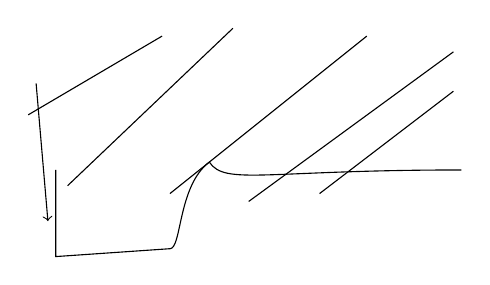
\begin{tikzpicture}[x=1cm,y=1cm]
\draw (0,2.5)--(1.7,3.5);\draw (.5,1.6)--(2.6,3.6);\draw (1.8,1.5)--(4.3,3.5);\draw (2.8,1.4)--(5.4,3.3);\draw (3.7,1.5)--(5.4,2.8);
\draw[->] (.1,2.9)--(.25,1.15);
\draw (.35,1.8)--(.35,.7)--(1.8,.8)..controls(1.95,.8)and(1.9,1.6)..(2.3,1.9)..controls(2.5,1.6)and(3,1.8)..(5.5,1.8);
\end{tikzpicture}}

Autodualité de la Jacobienne, suivant Artin-Mazur.
\margin{81}

\scanpage{83}
\uline{Cas de dim. relative 1}

Supposons \deleted{\unsure{que}} $X$ coho plat en dim $0$ i.e. $\mathrm H^0(X_s,\mathcal O_{X_s})\simeq\kappa(s)$.

Posons $P'=\operatorname{Ker}(P\xrightarrow{\deg}\mathbf Z_S)$\qquad $Q'=\operatorname{Ker}(Q\xrightarrow{\deg}\mathbf Z_S)$

On a un diagramme commutatif de suites exactes de faisceaux fppf
\diagram{\begin{tikzcd}
&0\arrow[d]&0\arrow[d]&0\arrow[d,no head]&\\
0\arrow[r,no head]&\Phi\arrow[r]\arrow[d]&P^0\arrow[r]\arrow[d]&Q^0\arrow[r,no head]\arrow[d,no head]&0\\
0\arrow[r,no head]&E\arrow[r]\arrow[d]&P'\arrow[r]\arrow[d]&Q'\arrow[r]\arrow[d]&0\\
0\arrow[r]&E/\Phi\arrow[r]\arrow[d]&E^*\arrow[r]\arrow[d]&\Psi\arrow[r,no head]\arrow[d]&0\\
&0&0&0&
\end{tikzcd}}
$E,E^*,\Phi,\Psi$ sont \deleted{des \unsure{schémas en gr.}}\inserted{\unsure{loc. ét. (sur $S$)}} représentables par des schémas en groupes \uline{étales}. Leurs fibres génériques est le groupe unité. Les fibres spéciales, si $\kappa(s)$ sép. clos, sont données par
\[
\Phi_{\unsure{(s)|(\bar s)}}=\operatorname{Ker}u\simeq\mathbf Z/d\mathbf Z,\qquad
\Psi_{\unsure{(s)|(\bar s)}}=\operatorname{Coker}u\qquad(d=\operatorname{pgcd}(d_i))
\]
où
\[
u:E_{(s)}\longrightarrow E^*_{(s)}
\]
est l'hom compris en diagramme.
\diagram{\begin{tikzcd}
0\arrow[r]&\mathbf Z\arrow[r,"\lambda=(d_i)"]&\mathbf Z^r\arrow[r,"\alpha"]&E_{(s)}\arrow[r]\arrow[d,dashed,"u"]&0\\
\deleted{\unsure{0}}&\mathbf Z\arrow[l,draw=none,"\deleted{\longleftarrow}" description]&\mathbf Z^r\arrow[l,"\mu:(d_i\delta_i)=(d_i^t)"']&E^*_{(s)}\arrow[l,"\beta"']&0\arrow[l]
\end{tikzcd}}
et
\[
(\beta\circ\alpha)((n_i)_i)=\left(\sum_{1\le i\le r}n_i(C_i,C_j)/\delta_j\right)_{1\le j\le r}.
\]
\margin{On a, si $X_{\widetilde s}$ est loc. fact.}
\margin{N.B. $E_{(s)}\simeq E(S)\longrightarrow P'(S)$ est donné par son composé avec $\alpha$, qui est $(n_i)\longmapsto\operatorname{cl}\mathcal O_X(\sum n_i C_i)$.
$P'(S)\longrightarrow E^*_{(s)}\simeq E^*(S)$ est donné par son composé avec $\beta$, qui est
$\mathcal L\longmapsto((\deg_{\kappa(s)}\mathcal L|C_i)/\delta_i)_i$.}
\figure{\begin{tikzpicture}[x=1cm,y=1cm]\draw (0,2.8)--(3.7,3.15);\draw (0,2.65)--(.05,.45)..controls(.1,.15)and(.8,.05)..(1.1,0)..controls(2,.05)and(2.8,.3)..(3.7,.3);\end{tikzpicture}}
\deleted{Lorsque $X$ vérifie \unsure{$N$}, alors $\Psi_{(s)}$ est aussi un groupe fini.}

Si \deleted{$\kappa(s)$ est parfait ou $(d^t,p)=1$, \unsure{ou que}} les anneaux locaux de $X_{\widetilde s}$ factoriels, alors $\Psi_{\unsure{s|(s)}}$ est aussi un groupe fini\inserted{(comme $\Phi_s$)},
\deleted{Si les anneaux locaux de $X_{\widetilde s}$ sont factoriels, \unsure{puisque dim $X_s=1$}, alors}
\inserted{Si de plus $\kappa(s)$ est parfait ou $(d^t,p)=1$, alors}
$Q'$ est un modèle de Néron de
\[
Q'_\eta=P'_\eta=P^0_\eta=\underline{\operatorname{Pic}}^0_{X_\eta/\kappa(\eta)}.
\]
En particulier, si $d^t=1$, donc $\Phi=0$, $Q'$ est un modèle de Néron de $\unsure{P^0_\eta}$, \unsure{enfin|et} $P'$ est (loc. ét) sur $S$ représentable.
\margin{82}

\scanpage{84}
N.B. Accouplons $\mathbf Z^r$ et $\mathbf Z^r$ par
\[
((n_i),(n'_i))=\sum\delta_i n_i n'_i
\]
Alors $\lambda$ et $\mu$ sont formellement transposés par cet accouplement,
\deleted{\unsure{parfait}}, donc $\operatorname{Ker}\mu\simeq E^*_{(s)}$ est accouplé à $\operatorname{Coker}\lambda\simeq E_{(s)}$, par la formule
\[
(\alpha(x),y^*)=(x,\beta y^*)\qquad x\in\unsure{\mathbf Z^r},\ y^*\in E^*_{(s)}.
\]
\[
E_{(s)}\times E^*_{(s)}\longrightarrow\mathbf Z
\]
\deleted{Par suite,} Je dis que l'on a aussi
\[
(x,u(y))=(y,u(x))\qquad\text{pour }x,y\in E_{(s)}.
\]
En effet, on peut supposer que
\[
x=\alpha(\underbrace{(n_i)}_{\underline n}),\quad y=\alpha(\underbrace{(n'_j)}_{\underline n'}),
\]
et les deux mbs sont resp.
\[
\begin{aligned}
(\alpha(\underline n),u(y))&=(\underline n,\beta u\alpha(\underline n'))\\
(\alpha(\underline n'),u(x))&=(\underline n',\beta u\alpha(\underline n))
\end{aligned}
\]
Or on a
\[
(\underline n,\beta u\alpha(\underline n'))=\sum n_i n'_j(C_i,C_j)
\]
qui est bien symétrique en \deleted{\unsure{et}} $\underline n,\underline n'$.

Si les $\delta_i$ sont tous $1$,\inserted{(p.ex $\kappa(s)$ p-fait)} alors on trouve pour l'accouplement précédent
\[
E^*_{(s)}\simeq\operatorname{Hom}(E_{(s)},\mathbf Z)
\]
et la \unsure{relation|dualité} symétrique si on a de plus $d=1$ i.e. $d^t=1$.
Dans ce cas cette dualité, et le fait que $u:E_{(s)}\unsure{-|\to}E^*_{(s)}$ est autoadjoint, donne pour le $\operatorname{Coker}u=\Psi_{(s)}$ une \uline{autodualité} canonique (à valeurs dans $\mathbf Q/\mathbf Z$). Cette autodualité \deleted{\unsure{est liée à}}\inserted{exprime} l'obstruction à étendre la biextension qu'on a de $(Q'_\eta,Q'_\eta)=(P^0_\eta,P^0_\eta)$ par $G_{m\eta}$, par une biextension de $Q',Q'$ par $G_m$.
\margin{\figure{\begin{tikzpicture}[x=1cm,y=1cm]
\node[draw,ellipse,align=center] (a) at (1.2,0) {modèles\\de Néron};
\draw[->] (.2,1)..controls(.2,.5)and(.4,.4)..(.65,.35);
\draw (.9,1)--(1.15,.45);
\end{tikzpicture}}}
\margin{83}

\scanpage{85}
\begin{center}
INSTITUT\\
DES HAUTES ETUDES SCIENTIFIQUES\\
91 - BURES-SUR-YVETTE\\
928 48-53
\end{center}
\margin{84.}

\cotefile{39}
\scanpage{3}
$k$ un \deleted{\unsure{corps commutatif avec}}\deleted{\inserted{\unsure{anneau}}} corps
\[
S_n(k)=k[[t_1,\ldots,t_n]]\qquad(n\ge0;\ S_0(k)=k)
\]
\margin{pour $n$ variable, on a un anneau cosimplicial}
$\mathcal A_n\subset S_n(k)$\qquad sous-anneau \unsure{cosimplicial|simplicial} i.e.

(b) $\forall n\ge0$, $\mathcal A_n$ est un sous-anneau unitaire de $S_n$

(a) On a

$a_1)$ $\mathcal A_n$ est st. par $\unsure{\mathfrak S_n|\mathcal S_n}$ opérant sur $S_n$

$a_2)$ Si $f(t_1,\ldots,t_n)\in\mathcal A_n$, alors $f(t_1,\ldots,t_n)\in\mathcal A_{n+1}$
\inserted{$t_{n+1}$ variable qui ne figure pas}

$a_3)$ Si $f(t_1,\ldots,t_n)\in\mathcal A_n$, alors $f(t_1,t_2,\ldots,\underbrace{t_{n-1},t_{n-1}}_{\text{répété}})\in\mathcal A_{n-1}$
\figure{\begin{tikzpicture}[x=1cm,y=1cm]\draw[->] (.5,2.5)..controls(-.4,2)and(-.3,.5)..(.3,.3)--(1,0);\end{tikzpicture}}
Le plus petit $\mathcal A_*=(\mathcal A_n)_{n\in\mathbf N}$ \deleted{\unsure{pareil}}\inserted{satisfaisant a) b)} est donné par \deleted{\unsure{$\mathcal A_*=P$}}
\[
\mathcal A_n=\operatorname{Im}(\mathbf Z\longrightarrow S_n)
\]
donc l'\deleted{objet}\inserted{anneau} cosimplicial constant de valeur $\operatorname{Im}(\mathbf Z\to k)$,
(qui est $\mathbf Z$ ou un $\mathbf Z/p\mathbf Z$, \deleted{\unsure{si $p>0$}}\inserted{$p$ nb premier} $=\operatorname{car}.k$)

On suppose de plus que

c) Si $f\in\mathcal A_n$\inserted{et} ($f\notin\operatorname{rad}S_n$, i.e. $f$ inv. dans $S_n$, alors $\frac1f\in\unsure{S_n|\mathcal A_n}$.
\[
\Updownarrow
\]
c') $\mathcal A_n$ est un anneau local, et l'inclusion $\mathcal A_n\to S_n$ est un hom local

Le plus petit $\mathcal A$ satisfaisant a) b) c) est formé des
\[
\mathcal A_n=\operatorname{Im}(P\longrightarrow S_n)
\]
où $P$ est le sous-corps premier de $k$ ($\mathbf Q$ en car $0$, $\mathbf F_p$ en car $p>0$).

d) $t_1\in\mathcal A_1\subset\unsure{S|k}[[t_1]]$

Le plus petit $\mathcal A$ satisfaisant à a) b) d) \deleted{\unsure{c)}} est formé des
\[
\mathcal A_n=P[t_1,\ldots,t_n]\deleted{\unsure{_{\mathfrak m_n}}}\qquad\deleted{\unsure{\mathfrak m_n=(}}
\]
le plus petit $\mathcal A$ satisfaisant a) b) c) d) est formé des
\[
\mathcal A_n=P[t_1,\ldots,t_n]_{\mathfrak m_n}\qquad\mathfrak m_n=\sum t_i P[t_1,\ldots,t_n].
\]
\deleted{\unsure{$\Phi$}}
Un hom $S_n\longrightarrow S_m$\inserted{ou $\underbrace{\operatorname{Spf}(S_m)}_{\Phi_m}\unsure{-|\to}\underbrace{\operatorname{Spf}(S_n)}_{\Phi_n}$}, donné par $f_1,\ldots,f_n\in S_m$ est dit un $\mathcal A$-hom si $f_1,\ldots,f_n\in\mathcal A_m$. Il résulte de b) et d) que l'identité $\Phi_n\longrightarrow\Phi_n$, \deleted{\unsure{et les applications}}\inserted{plus gén. les applications $\Phi_m\to\Phi_n$} sont des $\mathcal A$-hom (car $t_i\in\mathcal A_n$ pour $1\le i\le n$). L'analogue de b)
\margin{2}

\scanpage{4}
est la condition

e) Le composé de deux\inserted{$\mathcal A_*$} morphismes $X_m\unsure{-|\to}X_n\unsure{-|\to}X_p$ est un $\mathcal A_*$-morphisme.
\margin{Moyennant a) à e)}
\margin{$\operatorname{Hom}_{\mathcal A}(X_m,X_n)\unsure{\hookrightarrow|\longrightarrow}\operatorname{Hom}_{\mathcal A_0\text{-alg}}(\mathcal A_n,\mathcal A_m)$}
\figure{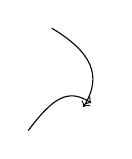
\begin{tikzpicture}[x=1cm,y=1cm]\draw[->] (0,1.3)..controls(.5,1)and(.65,.7)..(.4,.3);\draw[->](-.3,0)..controls(0,.4)and(.2,.55)..(.5,.35);\end{tikzpicture}}
\uline{NB} Moyennant \inserted{b) et} e), la condition a) équivaut au fait que
\[
\left\{\begin{array}{ll}
a_1)&1\in\mathcal A_0\\
a_2)&\text{le morphisme ``addition'' }X_1\times X_1\unsure{-|\to}X_1\text{ est }\mathcal A_*\text{-morph.}\\
a_3)&\rule{2.8cm}{0.3pt}\text{ ``produit'' }X_1\times X_1\unsure{-|\to}X_1\text{ est }\mathcal A_*\text{-morph.}
\end{array}\right.
\]
\uline{NB} Les $\mathcal A_n=k[t_1,\ldots,t_n]$ ou $\mathcal A_n=k[t_1,\ldots,t_n]_{\mathfrak m_n}$ satisfont e)

L'analogue de c) est la condition

f) Si $u:X_n\longrightarrow X_n$ est un $\mathcal A$-morphisme et un isomorphisme, \deleted{alors} i.e. le déterminant \deleted{\unsure{form}} de la matrice jacobienne de $u$ est inversible, alors $u^{-1}$ est un $\mathcal A$-morphisme

Cette condition implique \deleted{\unsure{(et est équivalente à f')}}

f') les $\mathcal A_n$ sont des anneaux henséliens,
\margin{f') implique-t-il f (moyennant a) à e))? il ne semble pas}

[En fait, si f) est satisfait pour un $n$, (f') est satisfait pour $n-1$, i.e. $\mathcal A_{n-1}$ est hensélien]

\deleted{D'ailleurs si $u:X_n\simeq X_n$ est donné par $f_1,\ldots,f_n\in\unsure{B_n|\mathcal A_n}$, alors $u^{-1}$ est donné par $g_1,\ldots,g_n$ appartenant à la clôture hensélienne de $(k[f_1,\ldots,f_n]_{\mathfrak m})$, où $\mathfrak m=k[f_1,\ldots,f_n]$}
\margin{\unsure{vicié?|inutile}}
\figure{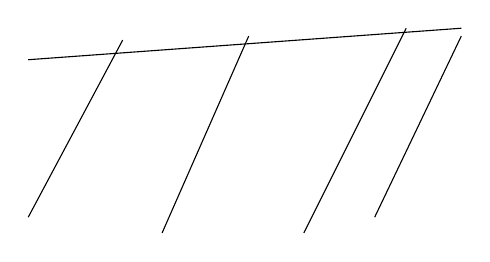
\begin{tikzpicture}[x=1cm,y=1cm]\draw(0,2)--(5.5,2.4);\draw(0,0)--(1.2,2.25);\draw(1.7,-.2)--(2.8,2.3);\draw(3.5,-.2)--(4.8,2.4);\draw(4.4,0)--(5.5,2.3);\end{tikzpicture}}
\uline{NB} Le plus petit $\mathcal A$ satisfaisant a) à d) et f') est formé des
\[
B_n=P\{t_1,\ldots,t_n\}\qquad\text{(clôture hensélienne des }P[t_1,\ldots,t_n]_{\mathfrak m_n}\text{)}
\]
et il satisfait $=$ e) et f).

\deleted{g) Soit $\xi$ un diag de variétés \unsure{for}}

Sous a) b) c) d) e) on définit la catégorie des $\mathcal A$-schémas formels,\inserted{et des Modules dessus (\unsure{finis de t.f.})} et le calcul différentiel dessus (opérateurs différentiels, parties principales,\inserted{\unsure{fibré tangent}} etc.\ $\ldots$)
\margin{(de préférence) \unsure{op. de passage aux produits fibrés} etc.\ $\ldots$}
\margin{3}

\scanpage{5}
Nous supposons maintenant $k$ de car. $0$, de sorte qu'on a la notion d'exponentielle d'un champ de vecteurs formel $\xi$, sur \deleted{\unsure{$X_n$}} un schéma. formel lisse $X$,
\[
(t,x)\longmapsto(\exp t\xi).x:\underset{\text{``axe temps''}}{\underline{X_1}}\times X\longrightarrow X
\]
\margin{Intégration d'équations différentielles}
g) Si $X$ est un $\mathcal A$-schéma formel (lisse) $\unsure{\xi|X}$ un\inserted{$\mathcal A_*$} champ de vecteurs, alors le résolvant $X_1\times X\unsure{-|\to}X$ est un $\mathcal A$-morphisme.

(Bien entendu, il suffirait de le \deleted{faire}\inserted{demander} pour $X$ de la forme $X_n\ldots$).

Ceci implique\inserted{et} (par l'\unsure{introd.} de la variable temps devenant variable spatiale), donc équivaut, à

g') Comme g), mais avec un ``champ de vecteurs variable avec le temps'' $\xi(t)$
(\diagram{\begin{tikzcd}
X_1\times X\arrow[r]\arrow[dr,dashed,"\operatorname{pr}_2"']&\underline{T(X)}\arrow[d,"p"']\\
&X
\end{tikzcd}}), on réslout l'équation différentielle formelle
\margin{variété \deleted{\unsure{des tangentes}}\inserted{formelle} tangente de $X$}
\[
\frac{d}{dt}x(t)=\xi(t,x)
\]
La résolution $x=\varphi(t,x_0)$ correspond à un $\varphi:X_1\times X\unsure{-|\to}X$ qui est un $\mathcal A$-morphisme.
\margin{4}

\scanpage{6}
\uline{Conséquence.} Soit $k_0=\mathcal A_0$, c'est un sous-corps de $k$. Soit $L(k_0)$ la catégorie des alg. de Lie de dim finie sur $k_0$. Par Hausdorff on a un foncteur
\[
L(k_0)\xrightarrow[\text{Hausdorff}]{}\operatorname{Grf}(k_0)\xrightarrow[\text{ext. de la base}]{}\operatorname{Grf}(k)
\]
où ``Grf'' désigne la \uline{catégorie des groupes formels}.
Ceci dit, ce foncteur se factorise canoniquement par les $\mathcal A$-groupes (formels) sur $k$. De façon plus précise, soit $\overline W(\unsure{V_0|\mathfrak g_0})$ le complété à l'origine \deleted{d'un}\inserted{de $V_0\otimes_{k_0}k$}\unsure{d'un} $k_0$-espace vectoriel\inserted{de dim finie} \deleted{\unsure{$V_0$}}. C'est un $\mathcal A$-schéma formel.
Les formules de Hausdorff, si $V_0$ est une Alg de Lie, définissent une loi de groupe
\[
\overline W(V_0)\times\overline W(V_0)\unsure{-|\to}\overline W(V_0)
\]
\uline{Cette dernière est une $\mathcal A$-loi}; \deleted{Pour ceci, il suffit de voir que le système de Pfaff associé est défini par une $\mathcal A$-loi\deleted{\inserted{\unsure{$\mathcal A$-forme}}}} et si
$V_0\unsure{-|\to}\unsure{\mathfrak h_0|h_0}$ est un hom d'algèbres de Lie sur $k_0$, l'hom de groupes formels $\overline W(V_0)\unsure{-|\to}\overline W(\mathfrak h_0)$ est un $\mathcal A$-hom.
Utilisant le th. d'\unsure{Ado|Abel}, on est ramené à prouver que si $V_0\subset\unsure{\mathfrak{gl}(n,k_0)|\mathfrak{gl}(n,k_0)_a}$, alors le sous-groupe formel de $\operatorname{Gl}(n,k_0)$ qu'il définit est un sous-$\mathcal A$-schéma formel $\ldots$
\margin{$-$}
\margin{5}

\scanpage{7}
\uline{Cor} $\mathcal A_1\subset S_1(k)$ stable par \unsure{primitivation} canonique (i.e. celle qui s'annule à l'origine), contient $\log(1+t_1)$, $\exp t_1$, $\cos t_1$, $\sin t_1$, $\operatorname{tg}t_1$ $\ldots$

Soit $X$ schéma. formel lisse de dim $n=p+q$. On sait ce que c'est qu'un \uline{feuilletage de $X$}\inserted{de dim $p$}, i.e. une variété formelle quotient $B$ de $X$, avec $X\unsure{-|\to}B$ submersif, $\dim B=q=n-p$. A un tel feuilletage $\varphi$ est associé un sous-module $\Phi\subset\Theta(X)$ [champs de vecteurs le long des fibres] qui est un ``système de Pfaff de dim $p$ complètement intégrable'', et réciproquement. Si $X$ est un $\mathcal A$-schéma, on dit qu'on a un $\mathcal A$-feuilletage si $\exists$\inserted{sur} $B$ une $\mathcal A$-structure (d'ailleurs unique\unsure{\}|)} grâce à f) telle que $X\longrightarrow B$ soit un $\mathcal A$-morphisme. Cela \uline{implique} que le sous-module $\Phi\subset\Theta(X)$ (ou sous-fibré de $T(X)$) soit un $\mathcal A$-sous-fibré -- i.e. qu'on ait un $\mathcal A$-syst. de Pfaff. compl. intégrable. On veut qu'on ait une réciproque, savoir

h) Si $\Phi_{\mathcal A}$ est un $\mathcal A$-syst. de Pfaff compl. intégrable sur un $\mathcal A$-schéma. formel $X$, alors il donne lieu à un $\mathcal A$-feuilletage \deleted{\unsure{compl. intégrable}}.
\margin{\uline{NB} h) implique g), qui équivaut à h) pour $p=1$}
\figure{\begin{tikzpicture}[x=1cm,y=1cm]\draw (0,2.4)..controls(1.1,3.2)and(1.6,2.4)..(.9,1.7)..controls(.5,1.2)and(.5,.5)..(0,.2);\end{tikzpicture}}
[En d'autres termes, si $i:Y\hookrightarrow X$ est un $\mathcal A$-morphisme donné tel que le composé
\[
T(Y)_0\xrightarrow{T(i)_0}T(X)_0\unsure{-|\to}T(X)_0/\Phi(0)
\]
soit un isom, alors l'unique morphisme
\[
\varphi:X\unsure{-|\to}Y
\]
tel que $\varphi\circ i=\operatorname{id}_Y$ et que $\varphi$ soit compatible avec $\Phi$, est un $\mathcal A$-morphisme $\ldots$

h') la fibre de $0$ dans un tel feuilletage est un sous-$\mathcal A$-variété formelle$\ldots$]
\figure{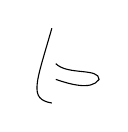
\begin{tikzpicture}[x=1cm,y=1cm]\draw (0,.8)..controls(-.2,.1)and(-.3,-.1)..(0,-.15);\draw (.05,.35)..controls(.2,.2)and(.6,.3)..(.6,.15)..controls(.5,0)and(.2,.1)..(.05,.15);\end{tikzpicture}}
\margin{6}

\scanpage{8}
\deleted{
\uline{Cor} $\mathcal A_1$ est stable par primitivation canonique (i.e. primitive d'augmentation nulle) contient $\log(1+t_1)$ (primitive de $\frac1{1+t_1}$) donc $\exp.t_1$ (série inverse), les fonctions $\cos t_1$, $\sin t_1$, $\operatorname{tg}t_1$ sont $\in\mathcal A_1$ $\ldots$

\uline{Lemme}\quad\deleted{\unsure{g) Soit}} Soit $X$ un\inserted{$\mathcal A$-} schéma formel (lisse)\inserted{de dim $n=p+q$}, $\Phi$ un ``système de Pfaff de degré $p$ complètement intégrable sur $X$'', \deleted{\unsure{$\Phi$}}
\deleted{\unsure{et un quotient}\quad \unsure{Soient} $Y,Z$ des schémas formels de dim $p$ resp $q$,
$f:X\to Y$ et $i:Z\to X$\inserted{des $\mathcal A$-morphismes}, tels que $T(p)(0)$ soit un \deleted{\unsure{isom}} $\Phi(0)\unsure{-|\to}T(Y)_0$ et que \deleted{\unsure{$T(i)(0)$}} le composé \deleted{\unsure{$T(X)_0$}}
\[
T(Z)_{\deleted{\unsure{(0)}}0}\overset{T(i)_0}{\unsure{-|\longrightarrow}}T(X)_{\deleted{\unsure{(0)}}0}\overset{\mathrm{can}}{\longrightarrow}T(X)_0/\Phi(0)
\]
soit un isom. On sait qu'il existe alors un isomorphisme\inserted{formel ($\varphi$ est néc. $\mathcal A$-isom)} unique
\[
X\overset{\varphi}{\simeq}Y\times Z
\]
\unsure{transformant $\Phi$ en produit} tel que $\operatorname{pr}_1\circ\varphi=p$, $\varphi\circ i=(z\mapsto(0,z))$)}

Soit $Z$\inserted{$\mathcal A$-} schéma formel\inserted{(lisse)} de dim $q$, $i:Z\unsure{-|\to}X$ une $\mathcal A$-immersion telle que le composé
\[
T(\unsure{Z|V})_0\overset{T(i)_0}{\unsure{-|\longrightarrow}}T(X)_0\longrightarrow T(X)_0/\Phi(0)
\]
soit un isom. On sait qu'il existe alors un unique morphisme formel
\[
X\xrightarrow{\pi}Z
\]
tel que $\pi\circ i=\operatorname{id}$, et que ``$\pi$ soit \deleted{\unsure{constant sur}}\inserted{compatible avec} le feuilletage défini par $\Phi$''. Conditions équivalentes

(i) $\pi$ est un $\mathcal A$-morphisme

(ii) $\exists$ $\mathcal A$-isom $X\simeq B\times Y$, tel que le feuilletage formel de $X$ défini par $\Phi$ soit le feuilletage défini par la projection $\operatorname{pr}_1:X\to B$. On dit
}
\figure{\begin{tikzpicture}[x=1cm,y=1cm]
\draw (.2,8)--(2.2,4.8)--(4.8,.3);\draw (2.4,7.9)--(5.3,4.6);\draw (4.6,7.7)--(5.7,5.2);\draw (0,6.2)--(0,4.1)..controls(0,4)and(.2,4)..(.3,4);\draw (0,6.5)--(5.8,6.45);\draw (.1,4.4)--(4.8,4.55);
\end{tikzpicture}}
\margin{7}

\scanpage{10}
$k$ anneau commutatif
\[
S_n=k[[t_1,\ldots,t_n]]\qquad(n\ge0)
\]
\[
X_n=\operatorname{Spf}(S_n)
\]
$X_*=(X_n)_{n\ge0}$ schéma formel simplicial augmenté

$S_*=(S_n)_{n\ge0}$ anneau top. cosimplicial coaugmenté

On suppose donné, pour tout $n$\inserted{$\ge0$}, un sous-ensemble $\mathcal A_n\subset S_n$

On pose $\mathcal A_*=(\mathcal A_n)_{n\ge0}$. Un morphisme $X_m\xrightarrow{p}X_n$, associé à un hom de $k$-algèbres topologiques $S_n\xrightarrow{p^*}S_m$, est dit un \uline{$\mathcal A_*$-morphisme} si $p^*(t_i)=f_i\in S_m$ est $\in\mathcal A_m$ pour tout $1\le i\le n$.
\margin{\uline{NB} les $f_i$ sont tels que $\varepsilon(f_i)$ nilpotent}
\inserted{Donc ceci signifie que les $\operatorname{pr}_i\circ p$ $(1\le i\le n)$ sont des $\mathcal A_*$-morph.}
On suppose:

(a) Les opérations simpliciales entre les $X_n$ sont des $\mathcal A_*$-morphismes ($\Longleftrightarrow$ $\forall n\ge0$ et $1\le i\le n$ on a $t_i\in\mathcal A_n$; $\Longleftrightarrow$ les morphismes identiques des $X_n$ sont $\in\unsure{\mathcal A_n|\mathcal A_*}$)
\margin{Identités}

(b) Le composé de deux $\mathcal A_*$-morphismes est \unsure{Itou|un}
\margin{Composition}
[$\Longleftrightarrow$ si $p:X_m\longrightarrow X_n$ est un $\mathcal A_*$-morphisme, alors $p^*(\mathcal A_n)\subset\mathcal A_m$ $\Longleftrightarrow$ si $f_1,\ldots,f_n\in\mathcal A_m$, et $\varepsilon(f_1),\ldots,\varepsilon(f_n)$ nilpotents, alors pour tout $\varphi\in\mathcal A_n$\inserted{avec $\varepsilon(\varphi)$ nilpotent}, on a $\varphi(f_1,\ldots,f_n)\in\mathcal A_m$]
\margin{NB \deleted{\unsure{Ceci devient vrai}}\unsure{moyennant c)}, vrai (sans supposer $\varepsilon(\varphi)$ nilpotent donc \unsure{$=$} si $a\in\mathcal A_0$, \unsure{du fait que} $\operatorname{Im}(\mathcal A_0\to S_n)\subset\mathcal A_n$)}
\figure{\begin{tikzpicture}[x=1cm,y=1cm]\draw(0,1.5)..controls(.5,1.8)and(.5,1.2)..(.8,1.2);\draw(.8,1.2)..controls(.6,.5)and(.7,0)..(0,-.4);\end{tikzpicture}}
\deleted{
(c) Le morphisme ``différence'' $X_2=X_1\mathbin{\widehat\times}_kX_1\longrightarrow X_1$ $((x,y)\mapsto x-y)$ et ``produit'' $[(x,y)\mapsto xy]$ sont des $\mathcal A_*$-morphismes [$\Longleftrightarrow t_1-t_2$ et $t_1t_2$ sont $\in\mathcal A_2$,\inserted{et $1\in\mathcal A_0$} $\Longleftrightarrow$ les $\mathcal A_n$ sont \deleted{stables par des additions et produits, \unsure{et par des différences}} \unsure{des sous-groupes abéliens stables par produit}] \unsure{$\mathcal A$}
\deleted{\unsure{$1\in S_0$}}
}
\inserted{[sous-anneaux unitaires des $S_n$]}
\margin{condition annulaire}
\figure{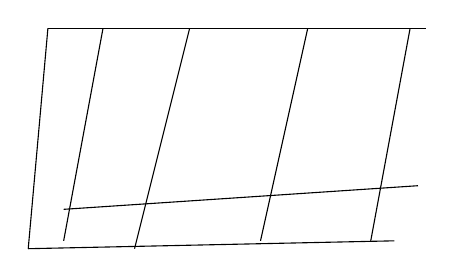
\begin{tikzpicture}[x=1cm,y=1cm]\draw(0,2.8)--(4.8,2.8);\draw(0,2.8)--(-.25,0);\draw(.7,2.8)--(.2,.1);\draw(1.8,2.8)--(1.1,0);\draw(3.3,2.8)--(2.7,.1);\draw(4.6,2.8)--(4.1,.1);\draw(-.25,0)--(4.4,.1);\draw(.2,.5)--(4.7,.8);\end{tikzpicture}}
\margin{9}

\scanpage{11}
\uline{NB} \deleted{Le plus petit $\mathcal A_*$}\inserted{a) b) c) impliquent} que $\mathcal A_*$ est un sous-anneau cosimplicial de $S_*$. Le plus petit $\mathcal A$ satisfaisant à a) b) c) est formé des
\[
\begin{aligned}
\mathcal A_n&=\operatorname{Im}(\mathbf Z[t_1,\ldots,t_n]\longrightarrow k[[t_1,\ldots,t_n]])\\
&\simeq\Lambda[t_1,\ldots,t_n]
\end{aligned}
\]
où
\[
\Lambda=\operatorname{Im}(\mathbf Z\longrightarrow k)\quad
\left\{\begin{array}{l}\simeq\mathbf Z\quad\text{ou}\\\simeq\mathbf Z/n\mathbf Z\quad\text{pour }n\in\mathbf N^*\ \text{conven.}\end{array}\right.
\]
Avec les conditions a) b) c) on construit la catégorie \deleted{\unsure{$\operatorname{Sfl}$}} $\operatorname{Sfl}_{\mathcal A_*}$ des \deleted{\unsure{$\mathcal A$}} schémas\inserted{$\mathcal A_*$} formels (lisses). Dans cette catégorie, il y a des produits finis ($X_n\simeq(X_1)^n$), et des produits fibrés, dans le cas ``transversal''.
\margin{Le foncteur ``oubli de $\mathcal A_*$'' commute à ces $\varprojlim$}
\inserted{Soit $k_0=\mathcal A_0\subset S_0\simeq k$.}
On obtient un foncteur $\mathbf V_{\mathcal A_*}$ de la co cat. des $k_0$-modules libres de t.f. (et $=$ projectifs de type fini?) vers les $\mathcal A_*$-schémas formels, par
\[
M_0\longmapsto\operatorname{Spf}\widehat{\operatorname{Sym}}^*_k(M_{0k})
\]
(où $M_{0k}=M_0\otimes_{k_0}k$). C'est $=$ un foncteur à valeurs dans les objets groupes de $\operatorname{Sfl}_{\mathcal A_*}$ i.e. vers les groupes $\mathcal A_*$-formels.
\margin{\deleted{\unsure{Nécessaire pour}\ \illegible{2}\ \unsure{obtenir un $\mathcal A$}\ \illegible{3}\ \unsure{par $\mathcal A$-morphismes}}}
\margin{\unsure{S'étend plus gén. aux modules de t. fini}\ $\ldots$}
\figure{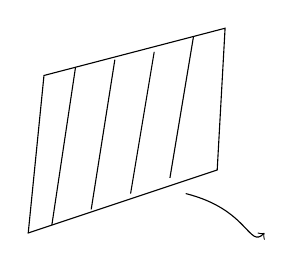
\begin{tikzpicture}[x=1cm,y=1cm]\draw(0,2)--(2.3,2.6)--(2.2,.8)--(-.2,0)--cycle;\draw(.1,.1)--(.4,2.1);\draw(.6,.3)--(.9,2.2);\draw(1.1,.5)--(1.4,2.3);\draw(1.6,.7)--(1.9,2.5);\draw[->](1.8,.5)..controls(2.6,.3)and(2.6,-.2)..(2.8,0);\end{tikzpicture}}
Plus \uline{gén.}, si $\unsure{\operatorname{Liss}(k_0)|\operatorname{Linc}(k_0)}$ est la catégorie des $k_0$-schémas \uline{augmentés}\inserted{$k_0$-}\unsure{morphismes} \deleted{\unsure{$\xi$}} des \deleted{\unsure{$\xi$}} $\operatorname{Sp}\operatorname{Sym}^*_{\unsure{k_0|k}}(M_0)$, \deleted{\unsure{on}} il y a un foncteur $X\unsure{-|\to}\widehat X^{(\mathcal A_*)}$ de $\unsure{\operatorname{Liss}(k_0)|\operatorname{Linc}(k_0)}$ vers les $\mathcal A_*$-schémas formels, commutant aux produits finis, et transformant objets groupes en objets groupes $\ldots$
\margin{$\mathcal O_{\mathcal A_*}(X)\subset\mathcal O(X)$.\quad
$\operatorname{Hom}_{\mathcal A_*\text{ form.}}\text{ ``}(X,X_1)\text{''}\quad \operatorname{Hom}_{k\text{-formel}}(X,X_1)$}
\margin{Modules \inserted{(lisses de t.f.)} $\mathcal A_*$ formels sur les schémas $\mathcal A_*$-formels$\ldots$\quad
\deleted{\unsure{Le sous}} fibré vectoriel $\mathcal A_*$ formel associé\quad
$\overline{\mathbf V}_{\mathcal A_*}(M)$, -- $W_{\mathcal A_*}(M)$}
\figure{\begin{tikzpicture}[x=1cm,y=1cm]\draw (0,5)--(0,2.5)..controls(.1,2.3)and(.2,2.3)..(.3,2.3)--(.3,.5)..controls(.3,.2)and(0,0)..(-.3,0);\draw[-](0,4.5)--(-.8,4.5);\end{tikzpicture}}
\margin{10}

\scanpage{12}
Les conditions a) b) c) sont les \uline{conditions logiques} élémentaires. On veut de plus

\margin{c) puis d) (condition différentielle)}
\unsure{d)|e)} (Condition hensélienne) Si $u:X_n\mathbin{-}X_n$ est un $A_*$-morphisme qui est un isomorphisme formel (i.e. si $f_1,\ldots,f_n\in A_n$ sont tels que $\varepsilon(f_1)\ldots\varepsilon(f_n)$ sont nilpotents dans $k$ et
\[
\varepsilon\left(\det\left(\frac{\partial f_i}{\partial\unsure{t_j|x_j}}\right)\right)
=\det\left(\varepsilon\left(\frac{\partial f_i}{\partial x_j}\right)\right)
=\det\left(\frac{\partial f_i}{\partial x_j}(0)\right)
\]
est un élément inv. de $k$) alors $u^{-1}$ est aussi un $A_*$-morphisme ($\Leftrightarrow$ le foncteur des $A_*$-schémas $A_*$ formels vers les schémas formels sur $k$ est conservatif).

\uline{Cor. 1} Si $f\in A_n$ et $f$ inversible dans $S_n$, i.e. $\varepsilon(f)=f(0)$ inversible dans $k$, alors $f^{-1}\in A_n$; \deleted{\unsure{f inversible|f même inversible}} si $f\in A_n$, $\varepsilon(f)=0$, alors $(1+f)^{-1}\in A_n$ ($\Leftrightarrow$ si $f\in A_n$ et $\varepsilon(f)=1$, alors $f^{-1}\in A_n$) $\Leftrightarrow A_n\cap\mathfrak m_n\subset\operatorname{rad}A_n$, où \deleted{$\unsure{\mathfrak m_n=}$} $\mathfrak m_n=(t_1,\ldots,t_n)S_n$ \deleted{\unsure{cas nilpotent de l'élément}}.
\margin{moyennant condition d) (différentielle)}

En effet, considérons le \deleted{\unsure{multi}} morphisme
\[
u:(x_1,\ldots,x_n,x_{n+1})\longmapsto
(x_1,\ldots,x_n,f(x_1,\ldots,x_n).x_{n+1})
\]
de $X_{n+1}$, il est un isom. formel d'inverse
\[
(x_1,\ldots,x_n,x_{n+1})\longmapsto
(x_1,\ldots,x_n,f(x_1,\ldots,x_n)^{-1}x_{n+1}),
\]
et comme \deleted{il} \inserted{$u$} est un $A_*$-morphisme, par d) il en est de $=$ de $u^{-1}$, donc
\[
g(t_1,\ldots,t_{n+1})=f(t_1,\ldots,t_n)^{-1}t_{n+1}\in A_{n+1},
\]
\deleted{i.e. $X_{n+1}\mathbin{-}X_1$ \unsure{comme}} donc $g(t_1,\ldots,t_n,1)\in A_n$ i.e. $f^{-1}\in A_n$. cqfd.
\margin{\unsure{ridicule avec la condition différentielle}}
\margin{incorrect, 1 n'est pas nilp.! Il faut exiger une propriété de divisi-bilité
\[
t_{n+1}f\in A_{n+1}\Longrightarrow f\in\unsure{A_{n+1}|A_n}
\]}
\figure{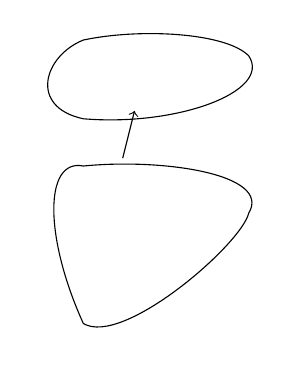
\begin{tikzpicture}[x=1cm,y=1cm]\draw (0,0) .. controls (-.7,.15) and (-.5,.8) .. (0,1) .. controls (.7,1.15) and (1.8,1.1) .. (2.1,.8) .. controls (2.4,.35) and (1.2,-.1) .. (0,0);\draw[->] (.5,-.5)--(.65,.1);\draw (0,-.6) .. controls (-.5,-.5) and (-.5,-1.5) .. (0,-2.6) .. controls (.5,-2.9) and (2,-1.6) .. (2.1,-1.2) .. controls (2.4,-.7) and (1,-.5) .. (0,-.6);\end{tikzpicture}}

\uline{Cor. 2} Soit \inserted{$P(Z)=$} $Z^N+f_1Z^{N-1}+\cdots+f_N\in A_n[Z]$ polynôme unitaire, soit $\zeta\in k_0$ tel que
\[
P^\varepsilon(\zeta)=\zeta^N+a_1\zeta^{N-1}+\cdots+a_N=0,
\quad\text{où les }a_i=\varepsilon(f_i)=f_i(0)\in k_0,
\]
\mspage{11}

\scanpage{13}
et $(P^\varepsilon)'(\zeta)=N\zeta^{N-1}+(N-1)a_1\zeta^{N-2}+\cdots+a_{N-1}$ soit $\in k^*$ (donc en fait $\in k_0^*$), de sorte qu'il existe une unique $F\in S_n$ telle que $P(F)=0$ et $\varepsilon(F)=\zeta$. Dans ces conditions, on a $F\in A_n$. [En d'autres termes, le couple $(A_n,\mu_n=\mathfrak m_n\cap A_n)$ est (non seulement \unsure{zariskien}, selon le cor. 1, mais même) hensélien]

\deleted{\unsure{Quitte à remplacer} $Z$ par $Z+\zeta$, SPS $\zeta=0$ donc $a_N=\varepsilon(f_N)=0$. En effet, on regarde $X_{n+1}\to X_{n+1}$ donné par
\[
(x_1,\ldots,x_n,x_{n+1})\longmapsto
(x_1,\ldots,x_n,x_{n+1}^{\unsure{N+1|N}}+f_1(x_1,\ldots,x_n)x_{n+1}\cdots)
\]
L'hyp. sur}
\figure{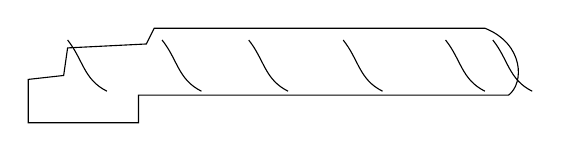
\begin{tikzpicture}[x=1cm,y=1cm]\draw (0,0)--(0,.55)--(.45,.6)--(.5,.95)--(1.5,1)--(1.6,1.2)--(5.8,1.2).. controls (6.3,1) and (6.3,.5)..(6.1,.35)--(1.4,.35)--(1.4,0)--cycle;\foreach \x in {.5,1.7,2.8,4,5.3,5.9}{\draw (\x,1.05) .. controls (\x+.2,.8) and (\x+.2,.55)..(\x+.5,.4);}\end{tikzpicture}}

Plus généralement

\uline{Cor 3} Soit $P\in A_{n+1}[t_1,\ldots,t_n,Z]$, $P=f_0+f_1Z+f_2Z^2+\cdots$ [les $f_i\in S_n(t_1,\ldots,t_n)$] supposons $\varepsilon(f_0)=0$ i.e. $\varepsilon(P)=0$, et $\varepsilon(f_1)\in k^*$ i.e. $\varepsilon\left(\frac{\partial P}{\partial Z}\right)\in k^*$, de sorte qu'il existe une unique $F\in S_n$ telle que $P(t_1,\ldots,t_n,F(t_1,\ldots,t_n))=0$ et $\varepsilon(F)=0$. Alors $F\in A_n$.

Soit en effet $u:X_{n+1}\mathbin{-}X_{n+1}$ donné par
\[
(x_1,\ldots,x_n,\zeta)\longmapsto(x_1,\ldots,x_n,P(x_1,\ldots,x_n,\zeta)),
\]
alors l'hyp. dit que c'est compatible avec les ponctuations, et que c'est un isomorphisme formel. Comme l'hyp. $P\in A_{n+1}$ implique $u$ un $A_*$-morphisme, $\unsure{u'|u^{-1}}$ est un $A_*$ morphisme et par suite $u^{-1}$ est un $A_*$-morphisme. Donc
\[
u^{-1}(x_1,\ldots,x_n,\zeta)=(x_1,\ldots,x_n,\deleted{\unsure{x}}\varphi(x_1,\ldots,x_n,\zeta))
\]
avec $\varphi\in A_{n+1}(t_1,\ldots,t_n,t_{n+1})$, donc $\inserted{F=}\varphi(t_1,\ldots,t_n,0)\in A_n(t_1,\ldots,t_n)$.
\margin{a) b) c) d) impliquent-ils que $S_n$ est fid. plat sur $A_n$ (si $k$ \deleted{\unsure{est}} l'est sur $k_0$)?}

\deleted{\unsure{d)|e)} (Condition différentielle) les $A_n$ sont stables par les opérateurs différentiels standards
\[
D_{\unsure{p_i|\underline p}}=D_{(p_1,\ldots,p_n)}
\left(=\frac{1}{p_1!\cdots p_n!}\frac{\partial^{|p|}}{\partial x_1^{p_1}\cdots\partial x_n^{p_n}}\right).
\]}
\figure{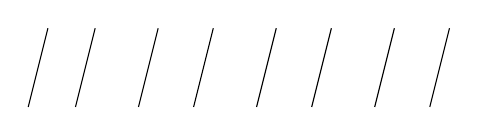
\begin{tikzpicture}[x=1cm,y=1cm]\foreach \x in {0,.6,1.4,2.1,2.9,3.6,4.4,5.1}{\draw (\x,0)--(\x+.25,1);}\end{tikzpicture}}
\mspage{12}

\scanpage{14}
Soient $X$ un schéma $A_*$-formel, et $Y$ un sous-schéma formel (lisse) de $X$. \deleted{On dit} On dit que $Y$ est un \deleted{sous} $A_*$-schéma $A_*$-formel s'il existe sur $Y$ une $A_*$ structure telle que l'inclusion can. soit un $A_*$-morphisme. Cette $A_*$-structure est alors unique. En effet, il est immédiat qu'on peut (sans hyp. sur $Y$) trouver un \inserted{$A_*$} morphisme $X\to Y'$ ($Y'$ un schéma $A_*$-formel) tel que le morphisme induit $Y\to Y'$ soit un isomorphisme formel. \deleted{\unsure{Considérons}} l'isomorphisme inverse, et le composé
\diagram{\begin{tikzcd}[column sep=small,row sep=tiny]&Y\arrow[dr,dash]&\\Y'\arrow[ur,"\sim"]\arrow[rr]&&X\end{tikzcd}}
Utilisant (e), on \deleted{\unsure{voit}} voit que \deleted{alors} $Y$ est un sous schéma $A_*$-formel ssi $Y'\mathbin{-}X$ est un $A_*$-morphisme, et alors la $A_*$-structure de $Y$ est celle déduite.

\uline{Exemple.} La diagonale de $X\times X$ est un sous $A_*$-schéma formel. Plus gén. celle de $X\times_Y X$ si $X\mathbin{-}Y$ est un $A_*$ morphisme submersif. \deleted{(i.e. \unsure{grad. tang.})}
\margin{Un morphisme formel $X\to Y$ entre sch. $A_*$-formels est un $A_*$-morphisme ssi son graphe dans $X\times Y$ est un sous-schéma $A_*$-formel.}
\figure{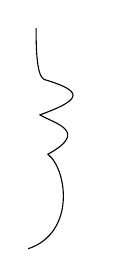
\begin{tikzpicture}\draw (0,0)..controls(.6,.2)and(.5,1)..(.25,1.2)..controls(.8,1.5)and(.3,1.6)..(.15,1.7)..controls(.7,1.9)and(.7,2)..(.2,2.15)..controls(.1,2.2)and(.1,2.6)..(.1,2.8);\end{tikzpicture}}

Soit $\mathfrak X$ un schéma sur $\mathcal O_{A_*}(X)$ ($X$ un $A_*$-schéma formel) muni d'une section \inserted{$s_0$} sur $\mathcal O_{A_*}(X)$, supposons que $\mathfrak X$ soit lisse sur $\operatorname{Spec}\mathcal O_{A_*}(X)$ aux points de cette section. Considérons le complété formel \inserted{$\hat{\mathfrak X}$} de $\mathfrak X\otimes_{\mathcal O_{A_*}(X)}\mathcal O(X)$ le long de la section $s$ déduite de $s_0$. Alors une constr. utilisant e) permet d'y mettre une \inserted{$A_*$-} structure, \inserted{telle que $X\to\hat{\mathfrak X}\mathbin{-}X$ soient des $A_*$-morphismes.} (\deleted{\unsure{Ce}} $\hat{\mathfrak X}$ est défini $A_*$-fonctoriellement dans le triple $(X,\mathfrak X,s_0)$, ce foncteur est compatible avec les images inverses par $X'\mathbin{-}X\ldots$)
\mspage{13}

\scanpage{15}
\inserted{(Condition différentielle)}
d) Tout $A_n$ est stable par les op. différentiels élémentaires $D_{\unsure{n|\underline n}}$ [$\Longrightarrow$ si $f(x_1,\ldots,x_n,y_1,\ldots,y_m)\in A_{n+m}$ est mis sous la forme $\sum_{p\in\mathbf N^m}f_p(x)y^p$, alors les $f_p$ sont $\in A_n$]
\margin{en car. 0 c'est équivalent à la stabilité par les $\frac{\partial}{\partial x_i}$.}
\figure{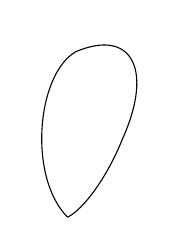
\begin{tikzpicture}\draw (0,0)..controls(-.5,.5)and(-.4,1.8)..(.1,2.1)..controls(.8,2.4)and(1.1,1.9)..(.7,1)..controls(.5,.5)and(.2,.1)..(0,0);\end{tikzpicture}}

Ceci implique que les algèbres $P^n_{X/k}$ sur $\mathcal O(X)$ ($X$ un \deleted{$A_*$} schéma $A_*$-formel) ont \deleted{une} $A_*$ structure canonique et fonctorielle, de $=$ $P^n_{X/Y}$ si $X\to Y$ est un $A_*$-morphisme submersif, de $=$ \deleted{\unsure{pour}} si $X\supset Y$ est un couple de schémas $A_*$-formels, $\mathcal O(Y)=\mathcal O(X)/J$, les \unsure{voisinages normaux|voisinages infinitésimaux} $\mathcal O_X/J^n$ ont des $A_*$-structures canoniques, fonctorielles, compatibles aux images inverses transversales. L'op. diff. universel d'ordre $n$
\[
\mathcal O(X)\mathbin{-}P^n_{X/k}
\]
\deleted{\unsure{est un} $A_*$ morphisme} applique $\mathcal O_{A_*}(X)$ dans $(P^n_{X/k})_{A_*}$ \deleted{$\unsure{\mathcal O_{A_*}}$} $\ldots\ldots$

\deleted{\unsure{Et}} Les $\operatorname{Diff}_n(X/k)$ (duals des $P^n_{X/k}$) ont \deleted{\unsure{une}} $A_*$-structures canoniques, leur composition \deleted{est} laisse stables les parties $\operatorname{Diff}_n(X_{A_*}/k)$ des $A_*$-op. diff., et ces derniers stabilisent les \deleted{$\unsure{A_*}$} $\mathcal O_{A_*}(X)\ldots\ldots$ Idem pour les op. diff. relatifs, pour $X\to Y$ $A_*$-morphisme \deleted{\unsure{étale}} \inserted{submersif}.

\uline{Cor} $A_n\subset k_0[[t_1,\ldots,t_n]]$. \deleted{\unsure{Les coefficients étant dans} $k_0$} D'où un foncteur $M_{A_*}$ des schémas $A_*$-formels vers les schémas formels sur $k_0\ldots$
\deleted{Soit $X\longrightarrow Y$ un morphisme submersif de schémas formels, sur $X$}
\figure{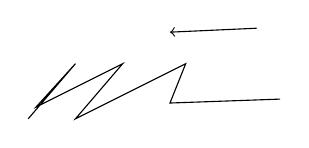
\begin{tikzpicture}[x=1cm,y=1cm]\draw (0,0)--(.6,.7)--(.1,.15)--(1.2,.7)--(.6,0)--(2,.7)--(1.8,.2)--(3.2,.25);\draw[<-] (1.8,1.1)--(2.9,1.15);\end{tikzpicture}}
\mspage{14}

\scanpage{16}
Soit $p:X\to Y$ un morphisme submersif de schémas formels (lisses), \unsure{supposons} $X$ muni d'une $A_*$-structure. On dit que $Y$ admet une $A_*$-structure quotient de celle de $X$ (moyennant $p$) s'il admet une \inserted{$A_*$} structure telle que $p$ devienne un $A_*$-morphisme. Celle-ci est encore unique: en effet, il existe (sans condition sur $Y$) un \deleted{\unsure{schéma}} sous-schéma $A_*$-formel $Y'$ de $X$, tel que le morphisme formel induit $Y'\to Y$ soit un isomorphisme. \deleted{Le} \inserted{Considérons le} composé
\diagram{\begin{tikzcd}[column sep=small,row sep=small]&Y\arrow[d,"\sim"]\\X\arrow[ur,dash,"p"]\arrow[r]&Y'\end{tikzcd}}
\deleted{\unsure{de $Y'$}}, on voit dès qu'à cs que la $A_*$-structure quotient existe ssi $\unsure{X'|X}\mathbin{-}Y'$ est un $A_*$-morphisme, et la $A_*$-structure sur $Y$ est celle déduite de celle de $Y'$.

\deleted{\unsure{Un cor}} Soit $X\xrightarrow{p}Y$ un morphisme formel submersif. Alors $R=X\mathbin{\hat\times}_Y X\subset X\mathbin{\hat\times}X$ est une \inserted{sous-schéma formel lisse, et c'est} relation d'équivalence [stable par symétrie, contient diagonale, transitif $\ldots$]. \deleted{\unsure{Inversement}} \inserted{Plus précisément} $X$ étant donné, il y a corr. biunivoque entre ces quotients formels $Y$, et les $R$ rel. d'équivalence formelles. Si $X$ est muni d'une $A_*$-structure, alors si $Y$ admet une $A_*$-structure quotient, on voit que $R$ est un sous-schéma $A_*$-formel de $X\mathbin{\hat\times}X$ i.e. il a une $A_*$-structure induite.

f) (Condition intégrale) La réciproque est vraie, i.e. si $R$ est une relation d'équival. formelle dans $X$, qui soit une \unsure{$A_*$-sous-structure|$A_*$-sous-schéma} de $X\mathbin{\hat\times}X$, alors
\mspage{15}

\scanpage{17}
le quotient \inserted{formel} $Y=X/R$ admet une $A_*$-structure quotient.

[Heuristiquement, étant donné un $A_*$-feuilletage de $X$, la variété formelle des feuilles admet une $A_*$-structure quotient. En car. 0, il est ``bien connu'' que les $A_*$-feuilletages correspondent aux ``systèmes de Pfaff complètement ``\uline{intégrables}'' sur $X$, et la ``condition intégrale'' signifie que l'intégration de ce système (effectuée disons, par le morphisme formel plus haut $X\mathbin{-}Y'$) se fait par un $A_*$-morphisme$\ldots\ldots$
\mspage{16}

\scanpage{19}
\uline{Th. de préparation ``formel''} Soit $A$ un anneau linéairement topologique, séparé et complet, $Z$ une indéterminée,
\[
F\deleted{(\unsure{Z})}=\sum_{i\geq0}a_iZ^i\in A[[Z]],\quad N\in\mathbf N\text{ tel que}
\]
i) $a_i$ est top.$^t$ nilpotent pour $0\leq i\leq N-1$

ii) $a_N$ est inversible

Alors $F$ est un élément \uline{régulier} de $A[[Z]]$ et $A[[Z]]/F$ a comme base $(Z^i)_{0\leq i\leq N-1}$, en d'autres termes tout élément $G$ de $A[[Z]]$ se met de façon unique sous la forme
\[
G=QF+\sum_{0\leq i\leq N-1}b_iZ^i\qquad
\begin{array}{l}Q\in A[[Z]]\\b_i\in A.\end{array}
\]

\uline{Démonstration} Comme $A$ est séparé et complet pour sa top. linéaire, on est ramené aussitôt au cas où $A$ est discret, alors i) \uline{signifie} que les $a_i$ ($0\leq i\leq\unsure{n|N}-1$) sont top. nilpotents. Soit $\mathfrak m$ l'idéal \inserted{(nilpotent)} qu'ils engendrent, $A_0=A/\mathfrak m$, et désignons par $\dot a_i,\dot F$ etc les réductions mod $\mathfrak m$. \deleted{\unsure{Alors}} Donc on a \deleted{$\unsure{\dot a}$}
\[
\dot a_i=0\quad\text{pour }0\leq i\leq N-1
\]
i.e.
\[
\dot F=\dot a_{N\deleted{\unsure{n}}}Z^{N\deleted{\unsure{n}}}+\cdots
=\dot a_{N\deleted{\unsure{n}}}Z^{N\deleted{\unsure{n}}}(1+\cdots)
\]
donc, comme $\dot a_{N\deleted{\unsure{n}}}$ est inversible par (ii), on voit que $\dot F$ est de la forme
\[
\dot F=\dot U Z^N.
\]
\deleted{\unsure{On voit donc}} donc
\[
\unsure{\dot A_0|A_0}[[Z]]/\dot F=A_0[[Z]]/Z^N\deleted{=A_0[Z]/Z^{\unsure{n|N}}}
\]
a comme base les $Z^i$ ($0\leq i\leq N-1$)

i.e.
\deleted{i) les $Z^i$ ($0\leq i\leq N-1$) engendrent $A[[Z]]/FA[[Z]]$.

En effet, ils engendrent mod $\mathfrak m$, on gagne donc par Nakayama.
\deleted{\unsure{Remarquons que}} \inserted{\unsure{le gr. associé de}} $A[[Z]]$ filtré $\mathfrak m$-adiquement \deleted{\unsure{par une}} \unsure{l'idéal}.

ii) $F$ est régulier. En effet, \unsure{a un gr. associé isomorphe à} $\unsure{\operatorname{Gr}_{\mathfrak m}^*(A)^{\mathbf N}|\operatorname{Gr}_{\mathfrak m}^*(A)[[Z]]}$.
\deleted{\unsure{de la nilpotence de} $\mathfrak m$, SPS $\mathfrak m=0$. Soit $Q\in A[[Z]]/\mathfrak m$ tel que $QF=0$, donc $\unsure{Q=0}$.}
Et l'opération de multiplication par $F$ dessus, sur le gradué associé: l'op. de multiplication par $\dot F$, qui est injective, OK.}
\figure{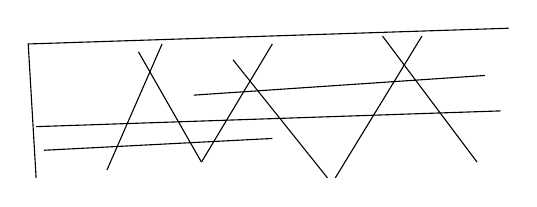
\begin{tikzpicture}[x=1cm,y=1cm]\draw (0,0)--(-.1,1.7)--(6,1.9);\draw (1.3,1.6)--(2.1,.2);\draw (1.6,1.7)--(.9,.1);\draw (2.5,1.5)--(3.7,0);\draw (3,1.7)--(2.1,.2);\draw (4.4,1.8)--(5.6,.2);\draw (4.9,1.8)--(3.8,0);\draw (2,1.05)--(5.7,1.3);\draw (0,.65)--(5.9,.85);\draw (.1,.35)--(3,.5);\end{tikzpicture}}
\mspage{18}

\scanpage{20}
\deleted{iii) Etude du cas où \deleted{$F\unsure{=}$} $a_i=0$ pour $i\geq N+1$, $a_N=1$.

i.e. du cas où
\[
F=Z^N+a_{N-1}Z^{N-1}+\cdots+a_0
\]
les $a_i$ ($0\leq i\leq\unsure{n|N}-1$) nilpotents.
\[
A[Z]/FA[Z]\longrightarrow A[[Z]]/FA[[Z]]
\]
\inserted{base $(Z^i)_{0\leq i\leq N-1}$ sur $A$}
est alors surjectif (car les $Z^i$ ($0\leq i\leq\unsure{n|N}-1$) engendrent $A[[Z]]/FA[[Z]]$ comme $A$-module) je dis que c'est bijectif i.e. que $(FA[[Z]])\cap A[Z]=FA[Z]$ (il revient au $=$ de dire que les \deleted{\unsure{éléments}} $Z^i$ ($0\leq i\leq\unsure{n|N}-1$) forment une base de $A[[Z]]/FA[[Z]]$).
\deleted{Soit donc $a_0+a_1Z+\cdots+a_{N-1}Z^{N-1}$ qui soit multiple de $F$ dans $A[[Z]]$ \unsure{on}.}}
\figure{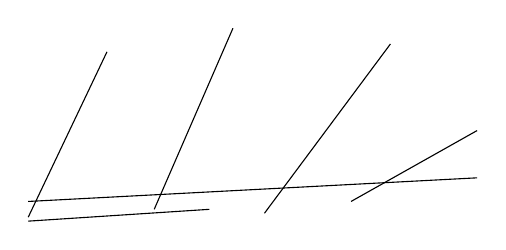
\begin{tikzpicture}[x=1cm,y=1cm]\draw (0,0)--(1,2.1);\draw (1.6,.1)--(2.6,2.4);\draw (3,.05)--(4.6,2.2);\draw (4.1,.2)--(5.7,1.1);\draw (0,.2)--(5.7,.5);\draw (0,-.05)--(2.3,.1);\end{tikzpicture}}

Considérons l'application
\[
\begin{aligned}
\varphi:\quad A^N+A[[Z]]&\longrightarrow A[[Z]]\\
((b_i)_{0\leq i\leq N-1},Q)&\mathbin{-}\sum_{0\leq i\leq N-1}b_iZ^i+QF
\end{aligned}
\]
l'application déduite par passage aux gradués associés pour la filtration $\mathfrak m$-adique (finie) est
\[
(\operatorname{Gr}A)^N\times(\operatorname{Gr}A)[[Z]]\mathbin{-}(\uline{\operatorname{Gr}A})[[Z]]
\]
donné pour un degré $n$ par
\[
((b_i),Q)\longrightarrow\sum_{0\leq i\leq N-1}b_iZ^i+Q\dot F
\]
et comme $\dot F=\deleted{\dot a_{\unsure{N+1|N-1}}}\alpha Z^N$ ($\alpha=\unsure{a_{N+1}|a_{N-1}}\in A_0^*$) ceci est manifestement bijectif, donc $\varphi$ aussi; cqfd.
\mspage{19}
